%!TEX root = ../thesis.tex
Our second prototype will move away from the world of jammable shape changing interfaces and into the surfaces of our environment.
Since the vision of ubiquitous computing was presented researchers have sought to integrate interactive technology into our everyday environment in variety of ways, which can be seen from the diverse selection of research fields that has stemmed from ubiquitous computing such as context awareness, tangible computing and shape changing interfaces.
In this prototype we have taken Weiser's vision very literally - how do you integrate interaction into the fabric of our everyday environment, i.e. the surfaces that surrounds us?

In the following sections we explore the possibilities of creating textile touch surfaces with advanced interaction capabilities as an exemplification of how surfaces can be used to interact in the home to create ad hoc interaction.
We have chosen to work with textiles as an interactive platform as we see unused potential in this area, both for its tangible and aesthetic textural qualities compared to e.g. polymer solutions \cite{rosenberg2009unmousepad}, as well as for the interesting possibilities to allow for DIY solutions to creating interactive surfaces in the home.

\todo{helt kort om hvad vi specifikt har lavet}

\section{Related work and approaches}
Before getting into detail with our implementation we will first give an overview of work and approaches that relates to our prototype and have inspired our solution.
We are, of course, not the first ones to consider the surfaces that surrounds us as interactive potential.
For example interactive floors such as iFloor \citep{petersen2005floor} and  iGameFloor \citep{gronbaek2007igamefloor}, augmented surface displays in fridges, walls and bowls \citep{taylor2007homes}, interactive tables such as reacTable \citep{jorda2007reactable} or, quite different from the other examples, REVEL that via a digital overlay changes the tactile perception of a physical surfaces \citep{bau2013revel}.

We have separated this section into three different fields that all have influenced the construction and implementation of our prototype work: electronic textiles, touch sensing and gesture recognition.
 
\subsection{Electronic Textiles}
\begin{quotation}
\emph{The most profound technologies are those that disappear. They weave themselves into the fabric of everyday life until they are indistinguishable from it. \citep{weiser1991computer}}
\end{quotation}
One of the research areas that have stemmed from ubiquitous computing is electronic textiles or `e-textiles', which seeks to integrate electronic and computation into fabric.
\citet{park2002wearable} presents the E-Textile vision as the paradigm the ``fabric is the computer'', taking Weiser's much quoted description of ubiquitous computing very literal.
One of the main obstacles for attaining this vision of the \emph{fabric as the computer} is how to incorporate the underlying computation into the fabric.
There are generally seen three ways to do it, either by computing \emph{offline}, on a separate system connected to the fabric, \emph{onto}, on components attached to the fabric or \emph{into} the fabric, embedded seamlessly into it \citep{marculescu2003}.
Today computation is commonly done either offline or onto the fabric, or a combination of the two, but advances in organic electronics and nano technology, for example with organic transistors weaved into fabric \citep{lee2005weave}, suggests that computation embedded into the fabric is not far off.

\begin{figure}[h]
\centering
\begin{minipage}{.3\textwidth}
  \centering
  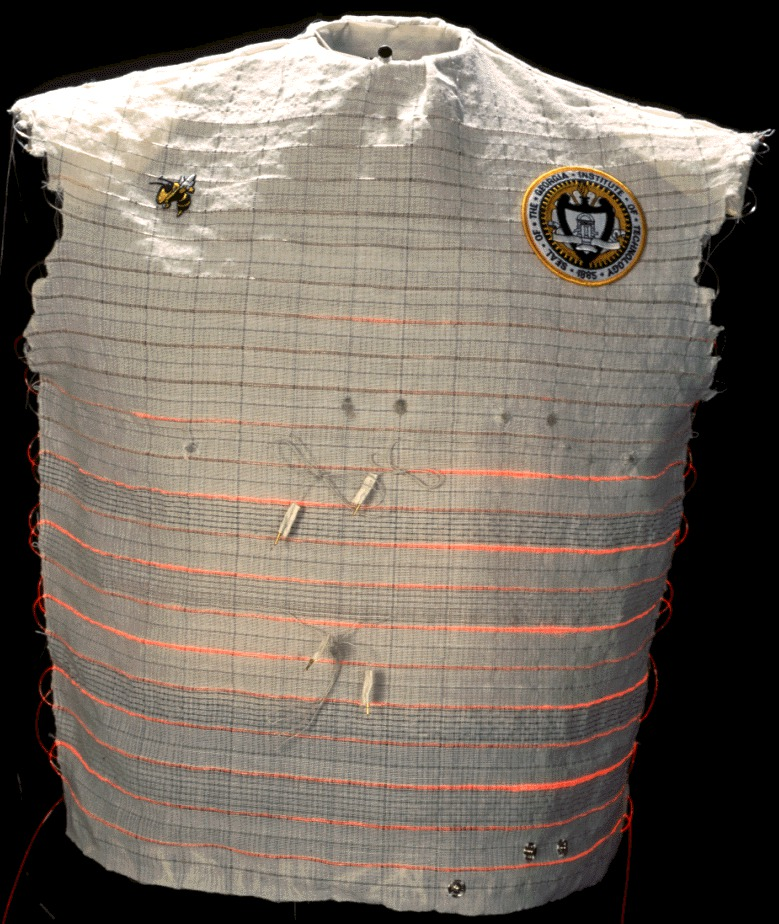
\includegraphics[width=0.8\linewidth]{figures/wearable_motherboard}
  \captionof{figure}{The Wearable Motherboard, taken from \citep{gopalsamy1999wearable}}
  \label{sofa_interaction:wearable_motherboard}
\end{minipage}%
\hspace{0.2cm}
\begin{minipage}{.3\textwidth}
  \centering
  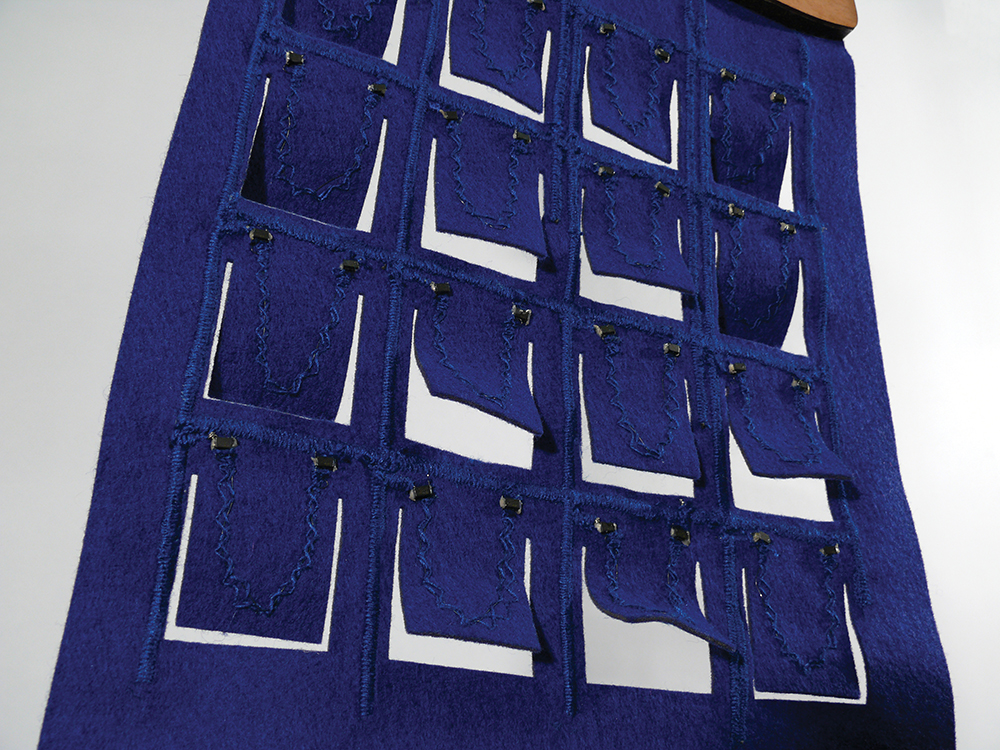
\includegraphics[width=0.8\linewidth]{figures/shutters}
  \captionof{figure}{Shutters, taken from \citep{coelho2009shutters}}
  \label{sofa_interaction:shutters}
\end{minipage}
\hspace{0.2cm}
\begin{minipage}{.3\textwidth}
  \centering
  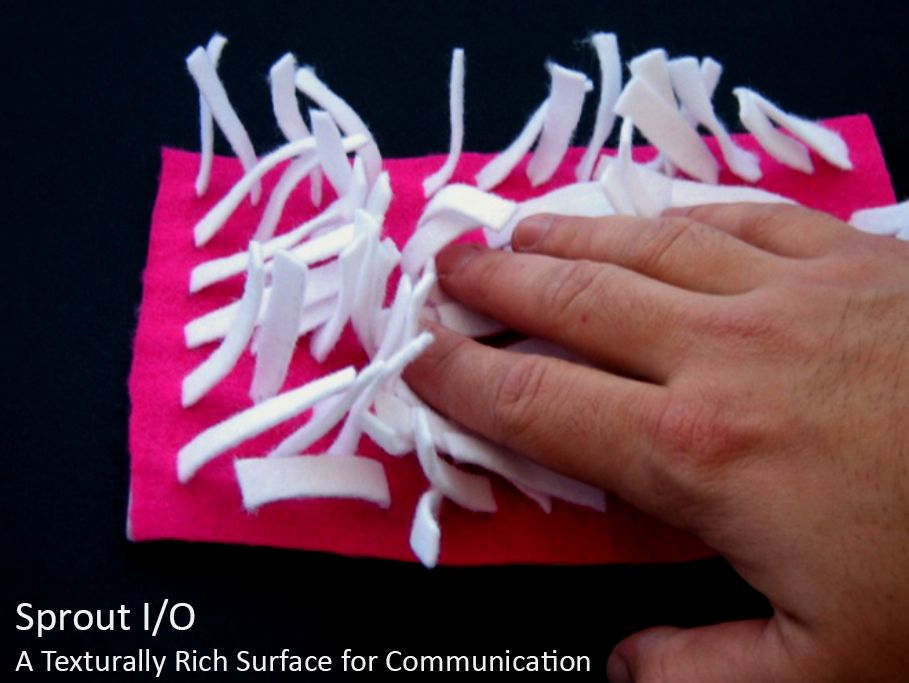
\includegraphics[width=0.8\linewidth]{figures/sprout}
  \captionof{figure}{Sprout I/O, taken from \citep{coelho2009shutters}}
  \label{sofa_interaction:sprout}
\end{minipage}
\end{figure}
E-textile is often seen used as part of wearable computing systems, logically, since clothing as a medium is ever present when people are involved.
An example of this is the Wearable Motherboard \citep{gopalsamy1999wearable} seen in figure~\ref{sofa_interaction:wearable_motherboard}, also called the ``Smart Shirt'', which is a lightweight monitoring `shirt' that can provide sensory data for use in medical and military contexts.
The fabric here is used as data paths that facilitates routing of information from any point to any other point on the shirt through conductive fibers embedded in the fabric.

E-textiles are not limited to wearable computing and clothing, and can just as well be part of interior design such as curtains, pillows, carpets, upholstery ect.
Shutters by \citet{coelho2009shutters}, seen in figure~\ref{sofa_interaction:shutters}, is an example of this where shape-memory alloy (SMA) threads are woven into a felt surface creating a curtain-like structure capable change of shape in permeability, used for indoor ventilation control among other things.
Here the SMA allows for actuation in the shutters while retaining the look, feel and softness of textile without any hard mechanic actuators.  
Another example from \citet{coelho2008sprout} is Sprout I/O, see figure~\ref{sofa_interaction:sprout}, where a membrane filled with strands of SMA and felt provides textually rich input and actuated output capabilities.
By measuring the capacitance between the users hand and the SMA threads touches can be registered, enabling stroke-like interaction, by creating an input matrix that register changes in each of the the individual SMA threads.

We have gotten a lot of inspiration from the various ``Do It Yourself'' (DIY) on-line communities related to e-textile craft and crafts in general, notably KOBAKANT DIY \citep{kobakantWEB} and Instructable \citep{instrucableWEB}.
Both sites provides guides, tips, and tricks for materials, construction and techniques and have for us been a good starting point for doing an e-textile project.
One of our inspirations has been rSkin \citep{rskinplusea,rSsininstructables}, a project by Hannah Perner-Wilson, which attempts to create a `skin' for a robot arm, made out of textiles, that enables the arm to register intensity and location of touches on the whole arm, seen in figure~\ref{rskin}.

\begin{figure}[hb]
	\centering
  		\includegraphics[width=3in]{figures/rskin}
	\caption[rSkin, Open Source Robot Skin]
   {rSkin, Open Source Robot Skin}
   \label{rskin}
\end{figure}
The `skin' is made of stretchy fabric and a 28 rows x 28 columns large pressure sensitive grid is embedded into the fabric using conductive thread.
The skin is made out of three layers: first a non-conductive layer with 28 rows of conductive thread, then a layer piezoresistive fabric and lastly a non-conductive layer with 28 columns of conductive thread.
The piezoresistive fabric acts as a pressure sensitive layer as piezoresistive materials decrease their electrical resistivity under mechanical stress \citep{piezoresistiveWIKIPEDIA}.
This approach to making pressure sensitive grids will be described in further detail in the implementation section as we use it as a starting point for our second prototype iteration.

\subsection{Touch Sensing}
\todo{bedre indledning}

Generally seen there are three broad categories for doing multi-touch input sensing: optical, capacitive and resistive \citep{rosenberg2009unmousepad}.

Optical sensing usually involve one or more digital cameras placed behind the touch surface to generate an image of the user's finger to track the interaction.
As this approach relies on cameras it is typically used for larger applications such as tabletops, since the cameras has to be far enough away to capture entire interactive surface, e.g. reacTable \citep{jorda2007reactable}, seen in figure~\ref{sofa_interaction:reactable} and the tabletop version of Microsoft Surface.

Capacitive sensing systems for touch based interaction rely on the human body's capacitive abilities to acquire the position of the touch on a surface. 
As a finger touches the surface, the surface's electrostatic field distorts and this change is then measurable as a change in capacitance at some position in a 2D grid.
The most common example of this approach is the touch surface of modern smart phones and tablets where touch has become the preferred form of interaction, for example Apples iPad seen in figure~\ref{sofa_interaction:ipad}.
Another example is Touch\'e \citep{sato2012touche} that allow objects and environments to become touch sensitive, allowing everyday objects to become touch interfaces, such as doorhandles, cups, water bottles ect.
This is done by sending a signal through the object and doing electromagnetic frequency sweeps. 
These frequencies will change when a touch occur and will change based on the size of the touched on the surface allowing for simple gesture recognition.
Two limitations of this technology is that pressure can not reliably be measured and that most systems based this technology only works with bare skin touching it.    

Resistive sensing is based on the principle of Force Sensitive Resistance (FSR).
The basic principle of a FSR sensor is to apply current to a semi-conductive material with piezoresistive capabilities then and read the outgoing current.
As stress is applied to the semi-conductor the resistance will decrease and the outgoing current will therefore increase. 
\citet{rosenberg2009unmousepad} describes FSR devices as 
\begin{quotation}
\emph{a continuous electrical switch through which electric conductance increases gradually as external force is applied}
\end{quotation}
The simple approach to making a touch sensetive surface, with multiple input areas, is to create a discrete array of FSR sensors in which each sensor has its own input and output channel.
This has some obvious limitations that will be discussed in iteration 1 in the next section.
Another approach is to create a row/column grid as seen in previously mentioned rSkin, this approach will be explored in iteration 2.
Lastly in iteration 3 we will explore the approach suggested by \citet{rosenberg2009unmousepad} to create a device based on IFSR, which is interpolating FSR, to increase the resolution of our prototype.
Generally seen resistive sensing is a low-cost and easy to implement solution to doing multi-touch interfaces and has the added benefit of being able to measure pressure.
It does also enable the use of flexible materials such as polymers in UnMousePad, seen wrapped on a coffee cup in figure~\ref{sofa_interaction:unmousepad}, and fabrics, as seen in rSkin where it is wrapped on a robot arm in figure~\ref{rskin}.
Though to attain resolutions higher than the size of the underlying grid, a lot of data processing has to be done as seen in \citep{rosenberg2009unmousepad}.
Also from our own experience with the technology we have seen a lot of input signal noise from the sensor which makes it harder to get accurate position tracking.   

\begin{figure}[h]
\centering
\begin{minipage}{.3\textwidth}
  \centering
  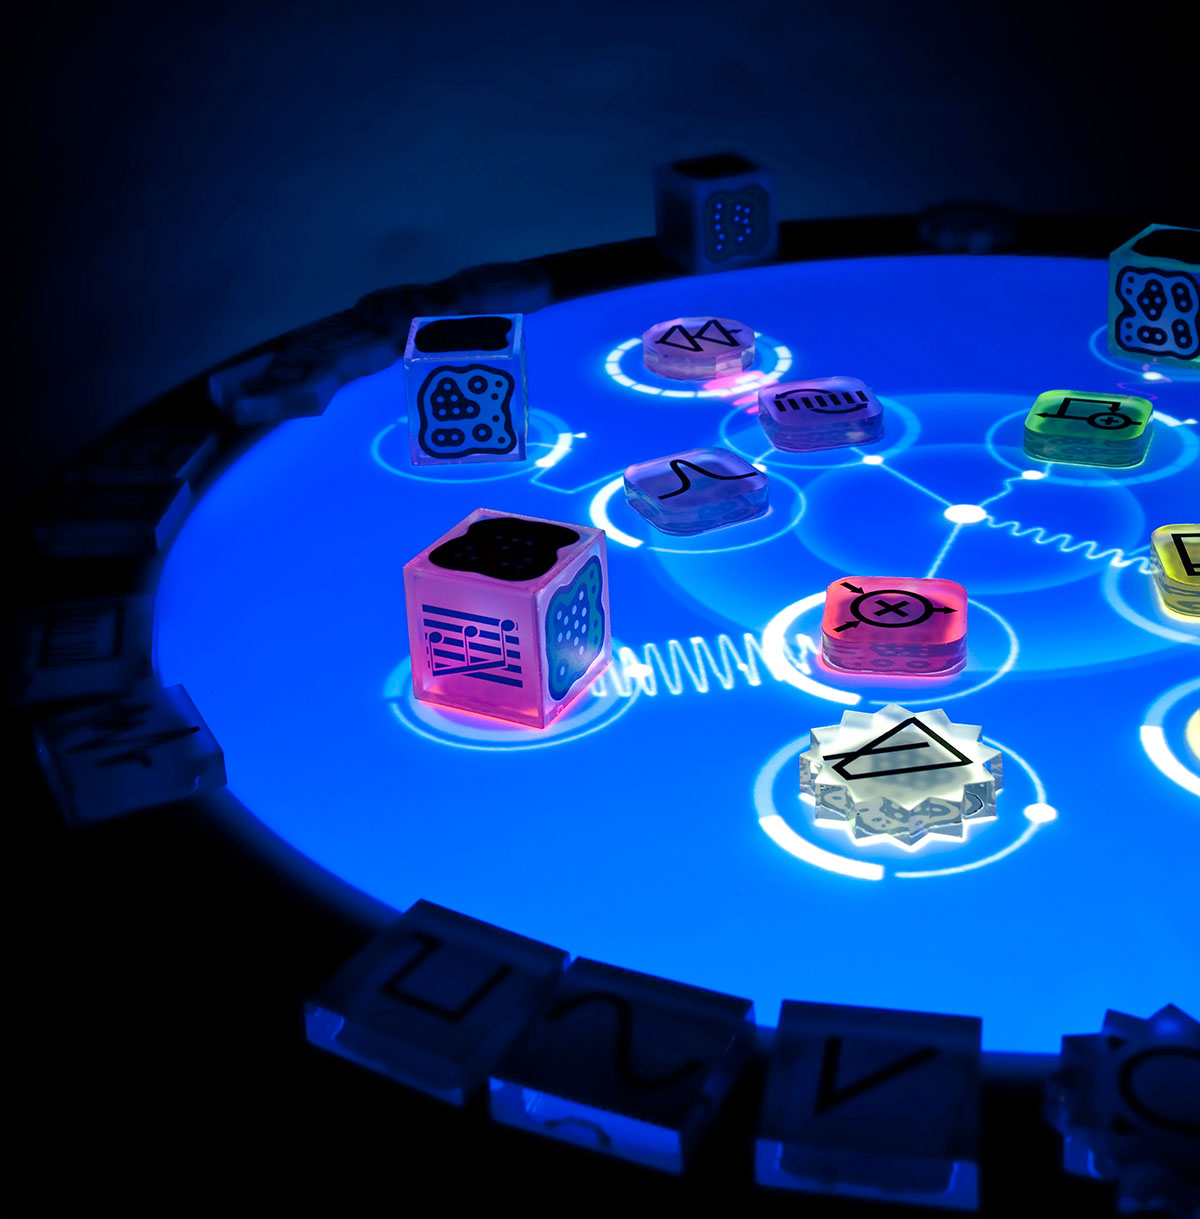
\includegraphics[width=0.8\linewidth]{figures/touch/reactable}
  \captionof{figure}{Example of an optical sensing system, reacTable}
  \label{sofa_interaction:reactable}
\end{minipage}%
\hspace{0.2cm}
\begin{minipage}{.3\textwidth}
  \centering
  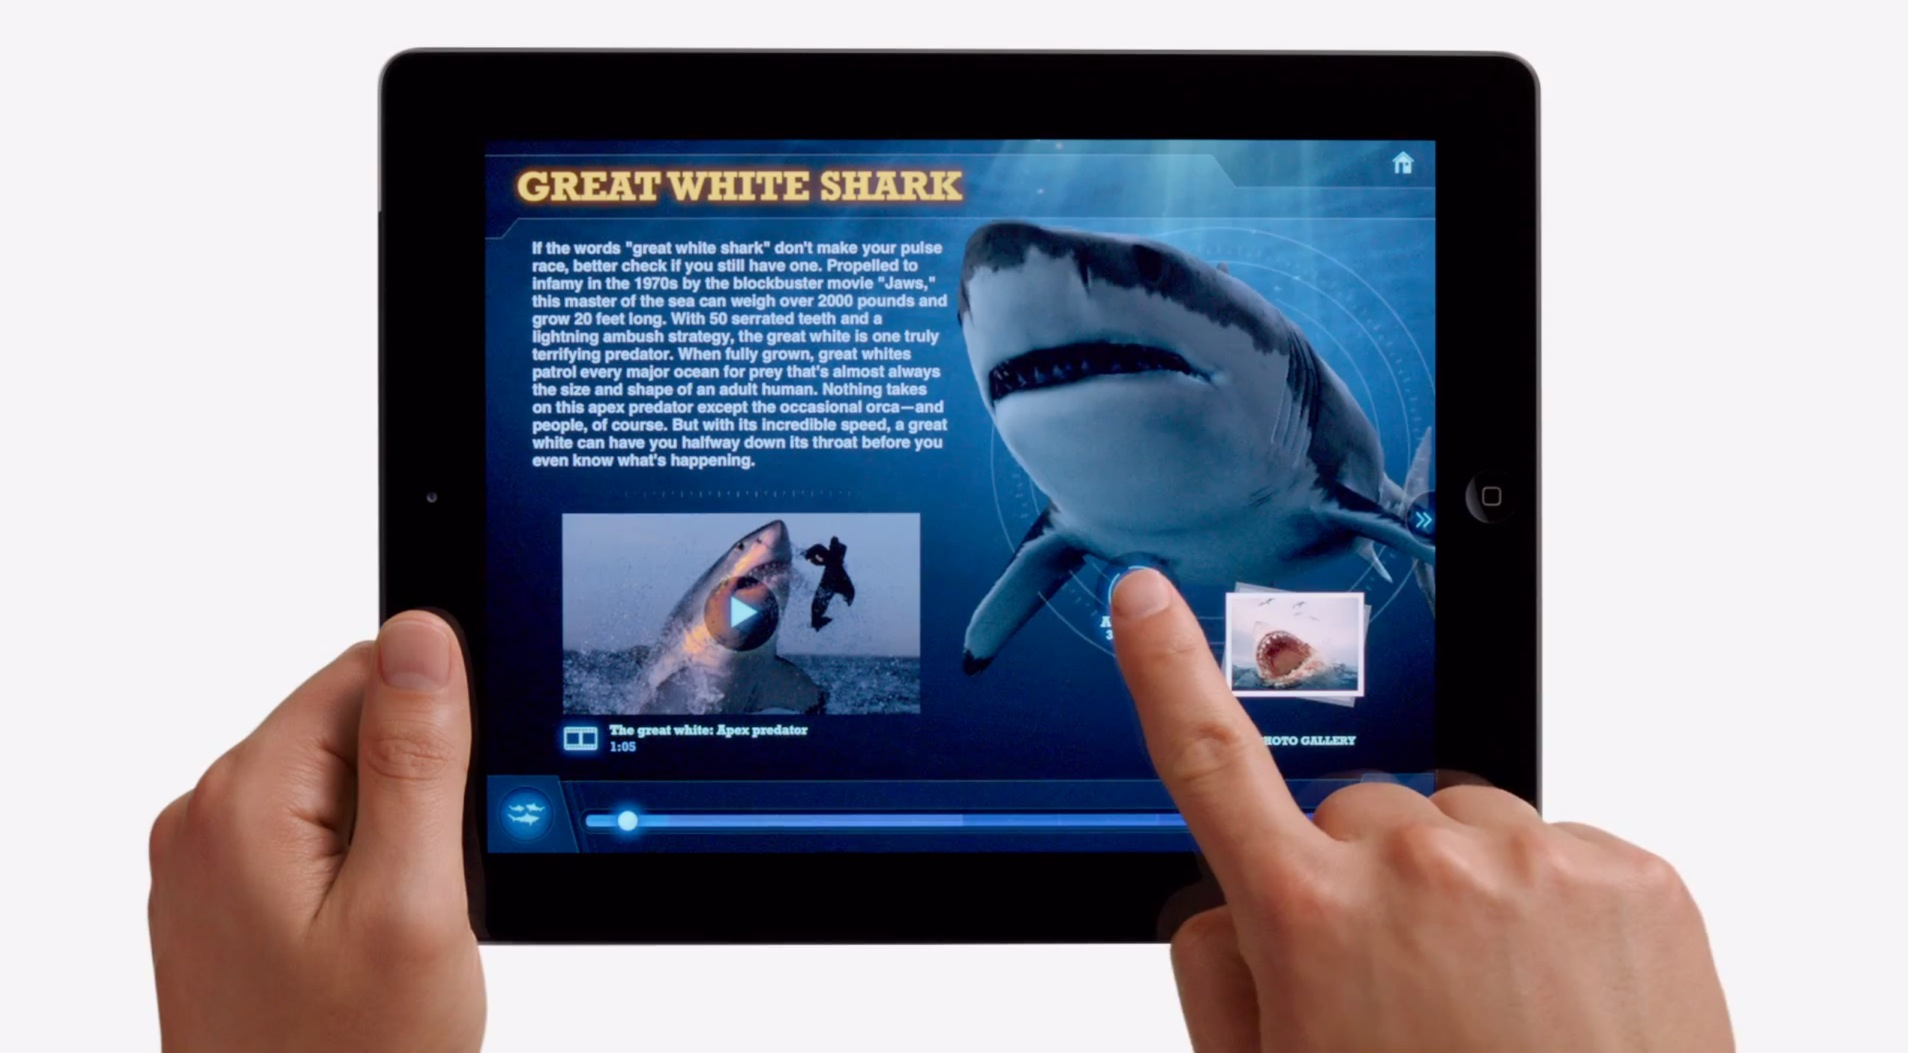
\includegraphics[width=0.8\linewidth]{figures/touch/ipad}
  \captionof{figure}{Example of a capacitive sensing system, iPad}
  \label{sofa_interaction:ipad}
\end{minipage}
\hspace{0.2cm}
\begin{minipage}{.3\textwidth}
  \centering
  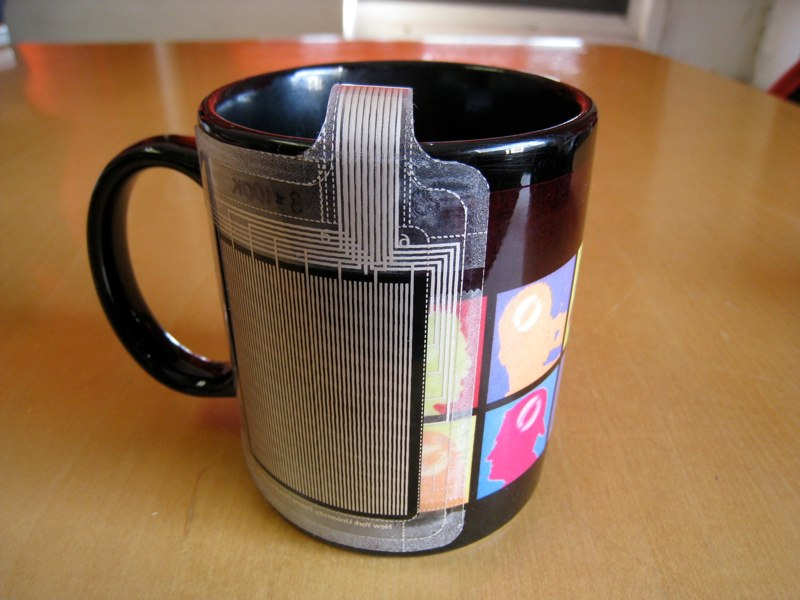
\includegraphics[width=0.8\linewidth]{figures/touch/unmousepad}
  \captionof{figure}{Example of a resistive sensing system, an UnMousePad sensor on a cup} 
  \label{sofa_interaction:unmousepad}
\end{minipage}
\end{figure}

\subsection{Gesture recognition}
Being able to sense a x-y position or a pressure map on an interactive surface is usually not enough for an application to provide interesting interaction possibilities.
Adding gestures can be one way to approach the interaction in a more involving, natural and expressive way.
\citet{baudel1993charade} points out three possible advantages in using gesture based systems:
\begin{itemize}
  \item \emph{Natural interaction:} Gestures are a natural and intuitive way to interact that is easy to learn.
  \item \emph{Terse and powerful interaction:} The expressive nature of a gesture can provide the ability for a single gesture to specify both a command and its parameters.
  \item \emph{Direct interaction:} As the hand is used for input no intermediate transducer is needed
\end{itemize}
Gestures inherent expressive character does pose a challenge though as the computer system has to interpret the gesture in some way to give it meaning.
Reversely the user needs to know, or at least have hints at, which gestures that the system understands in order to interact with it.
Some types of gestures and their interaction meaning has eventually become so common that their behaviour is expected when interacting with touch interfaces today, for example pinch for zoom out, inverse pinch for zoom in and horizontal swipes for shifting though pages.
A standardized interaction model for gesture interfaces are still a long way off though, at least in our opinion. 

The increase in mainstream use of touch input devices of various types and sizes such as tablets, tabletops and smart phones has resulted in some easily accessible frameworks for doing gesture recognition.
This is a relatively new thing as earlier gesture recognition was reserved for experts in pattern matching and therefore not quite suitable for user interface prototyping, unless you where able to put a large amount of work into it \citep{wobbrock2007gestures}.  

\todo{mere om dollar recognizers generelt}

The dollar family of recognizers \citep{anthony2010lightweight,vatavu2012gestures,wobbrock2007gestures} are some of the most popular frameworks for doing easily implementable 2-D gesture recognition.
This family of recognizers are all geometric template matchers which means that they match the user input against a predefined template, and based on an Euclidean distance scoring function, selects the best match between template and input.
\begin{itemize}
  \item \emph{\$1-recognizer \citep{wobbrock2007gestures}:} is a single-stroke recognizer, fast
  \item \emph{\$N-recognizer \citep{anthony2010lightweight}:} is a multi-stroke recognizer, slow
  \item \emph{\$P-recognizer \citep{vatavu2012gestures}:} is a single and multi-stroke point-cloud recognizer, faster than \$N
\end{itemize}
We have implemented and experimented with the \$N and \$P recognizer as to determine which one performs the best with our data input, this will be discussed in section \todo{ref til sektion}.

\todo{giver det mening at teste dollar-1?}

\section{Concept (el. Design Principles som i Coelho)}
%!TEX root = ../thesis.tex
The prototype that we have made for this chapter serves to exemplify both the qualities and possibilities of textile interfaces in general but also as an example of how surfaces in our environment can be enhanced and used in new ways for ad hoc interaction.
Our prototype is a generic touch surface meant to be integrated into the environment in various ways.
As the prototype has been made with textiles it is most suitable for textile based integrations such as furniture, sheets, cloth etc.
The technique used does however extend beyond the use of textiles and could just as well be implemented with other materials such as wallpaper, polymers, or printed circuit boards (PCB).

To explore more advanced touch interactions the prototype is programmed to recognise various gestures which we exemplify by a scenario of controlling existing devices of the home.
These gestures are then mapped to \todo{mangler noget}

%The scenarios which we have envisioned are focus around pervasive touch surfaces in the home environment for the control of existing devices.

\section{(Process and) Implementation}
%!TEX root = ../thesis.tex
This section will go though the process and implementation of our prototype.
\todo{As one of the goals of this prototype has been to implement advanced interaction possibilities into a textile surface without the use of advanced machinery ... something something}
To give an insight into the prototype process as well as the final prototype, we have chosen to split the implementation into three overall iteration steps.
Our hope is that this will give a better understanding of the rationale behind our construction decisions as well as ... something something 

\todo{iterationer skal indeholder motivation for n\ae ste skridt \dots}

\todo{iteration 1 is longer because we describes the basics osv. ??}

\subsection{Iteration 1}
\label{ch:textiletouch:it1}
The goal of our first iteration of the prototype was to ensure that the we had construction principles and the right materials for constructing a touch and pressure sensitive fabric, with only off-the-shelf materials and tools.

\subsubsection{Construction principles}
As a first iteration of our prototype we applied the principles from Pressure Sensor Matrix\footnote{http://www.instructables.com/id/Pressure-Sensor-Matrix/}, to construct a simple 2x3 touch pad in neoprene, seen in figure~\ref{prototype_1}, and a bend sensor for simple testing, also seen in figure~\ref{prototype_1}.
The prototype consists of three layers as depicted in figure~\todo{ref}, connected to an Arduino\footnote{http://www.arduino.cc/} for input/output data that is sent to Processing\footnote{http://processing.org/} for data visualization.

\begin{figure}[h]
  \centering
      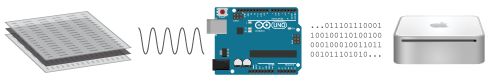
\includegraphics[width=\textwidth]{figures/touch/process}
  \caption{Data process}
   \label{data-process}
\end{figure}

The top layer is made of 3 mm thick neoprene from an old mouse pad with one long conductive thread, made of stainless steel fibers, sewn into it.
Neoprene is easy to work with and gives a natural force-feedback when touched because of its thickness, \hl{but lacks the naturalness and flexibility of normal fabric used for clothing}.
The middle layer made from anti-static polymer bags that are normally used to protect electronics. 
Some types of anti-static bags, such as the ones we have used, acts as semi-conductors with piezoresistive capabilities and therefore fits in a FSR sensor.
We have tested three different types of anti-static bags, two  transparent and one black, but only black ones are piezoresistive.
We do not know if this is the general case as we only had a limited number of samples.
The bottom layer is another layer of neoprene, but with separate conductive stitchings for each of the 2 x 3 cells.
The setup is illustrated in figure~\ref{layers_iteration1}.

\begin{figure}[h]
\centering
\begin{subfigure}[t]{.5\textwidth}
  \centering
  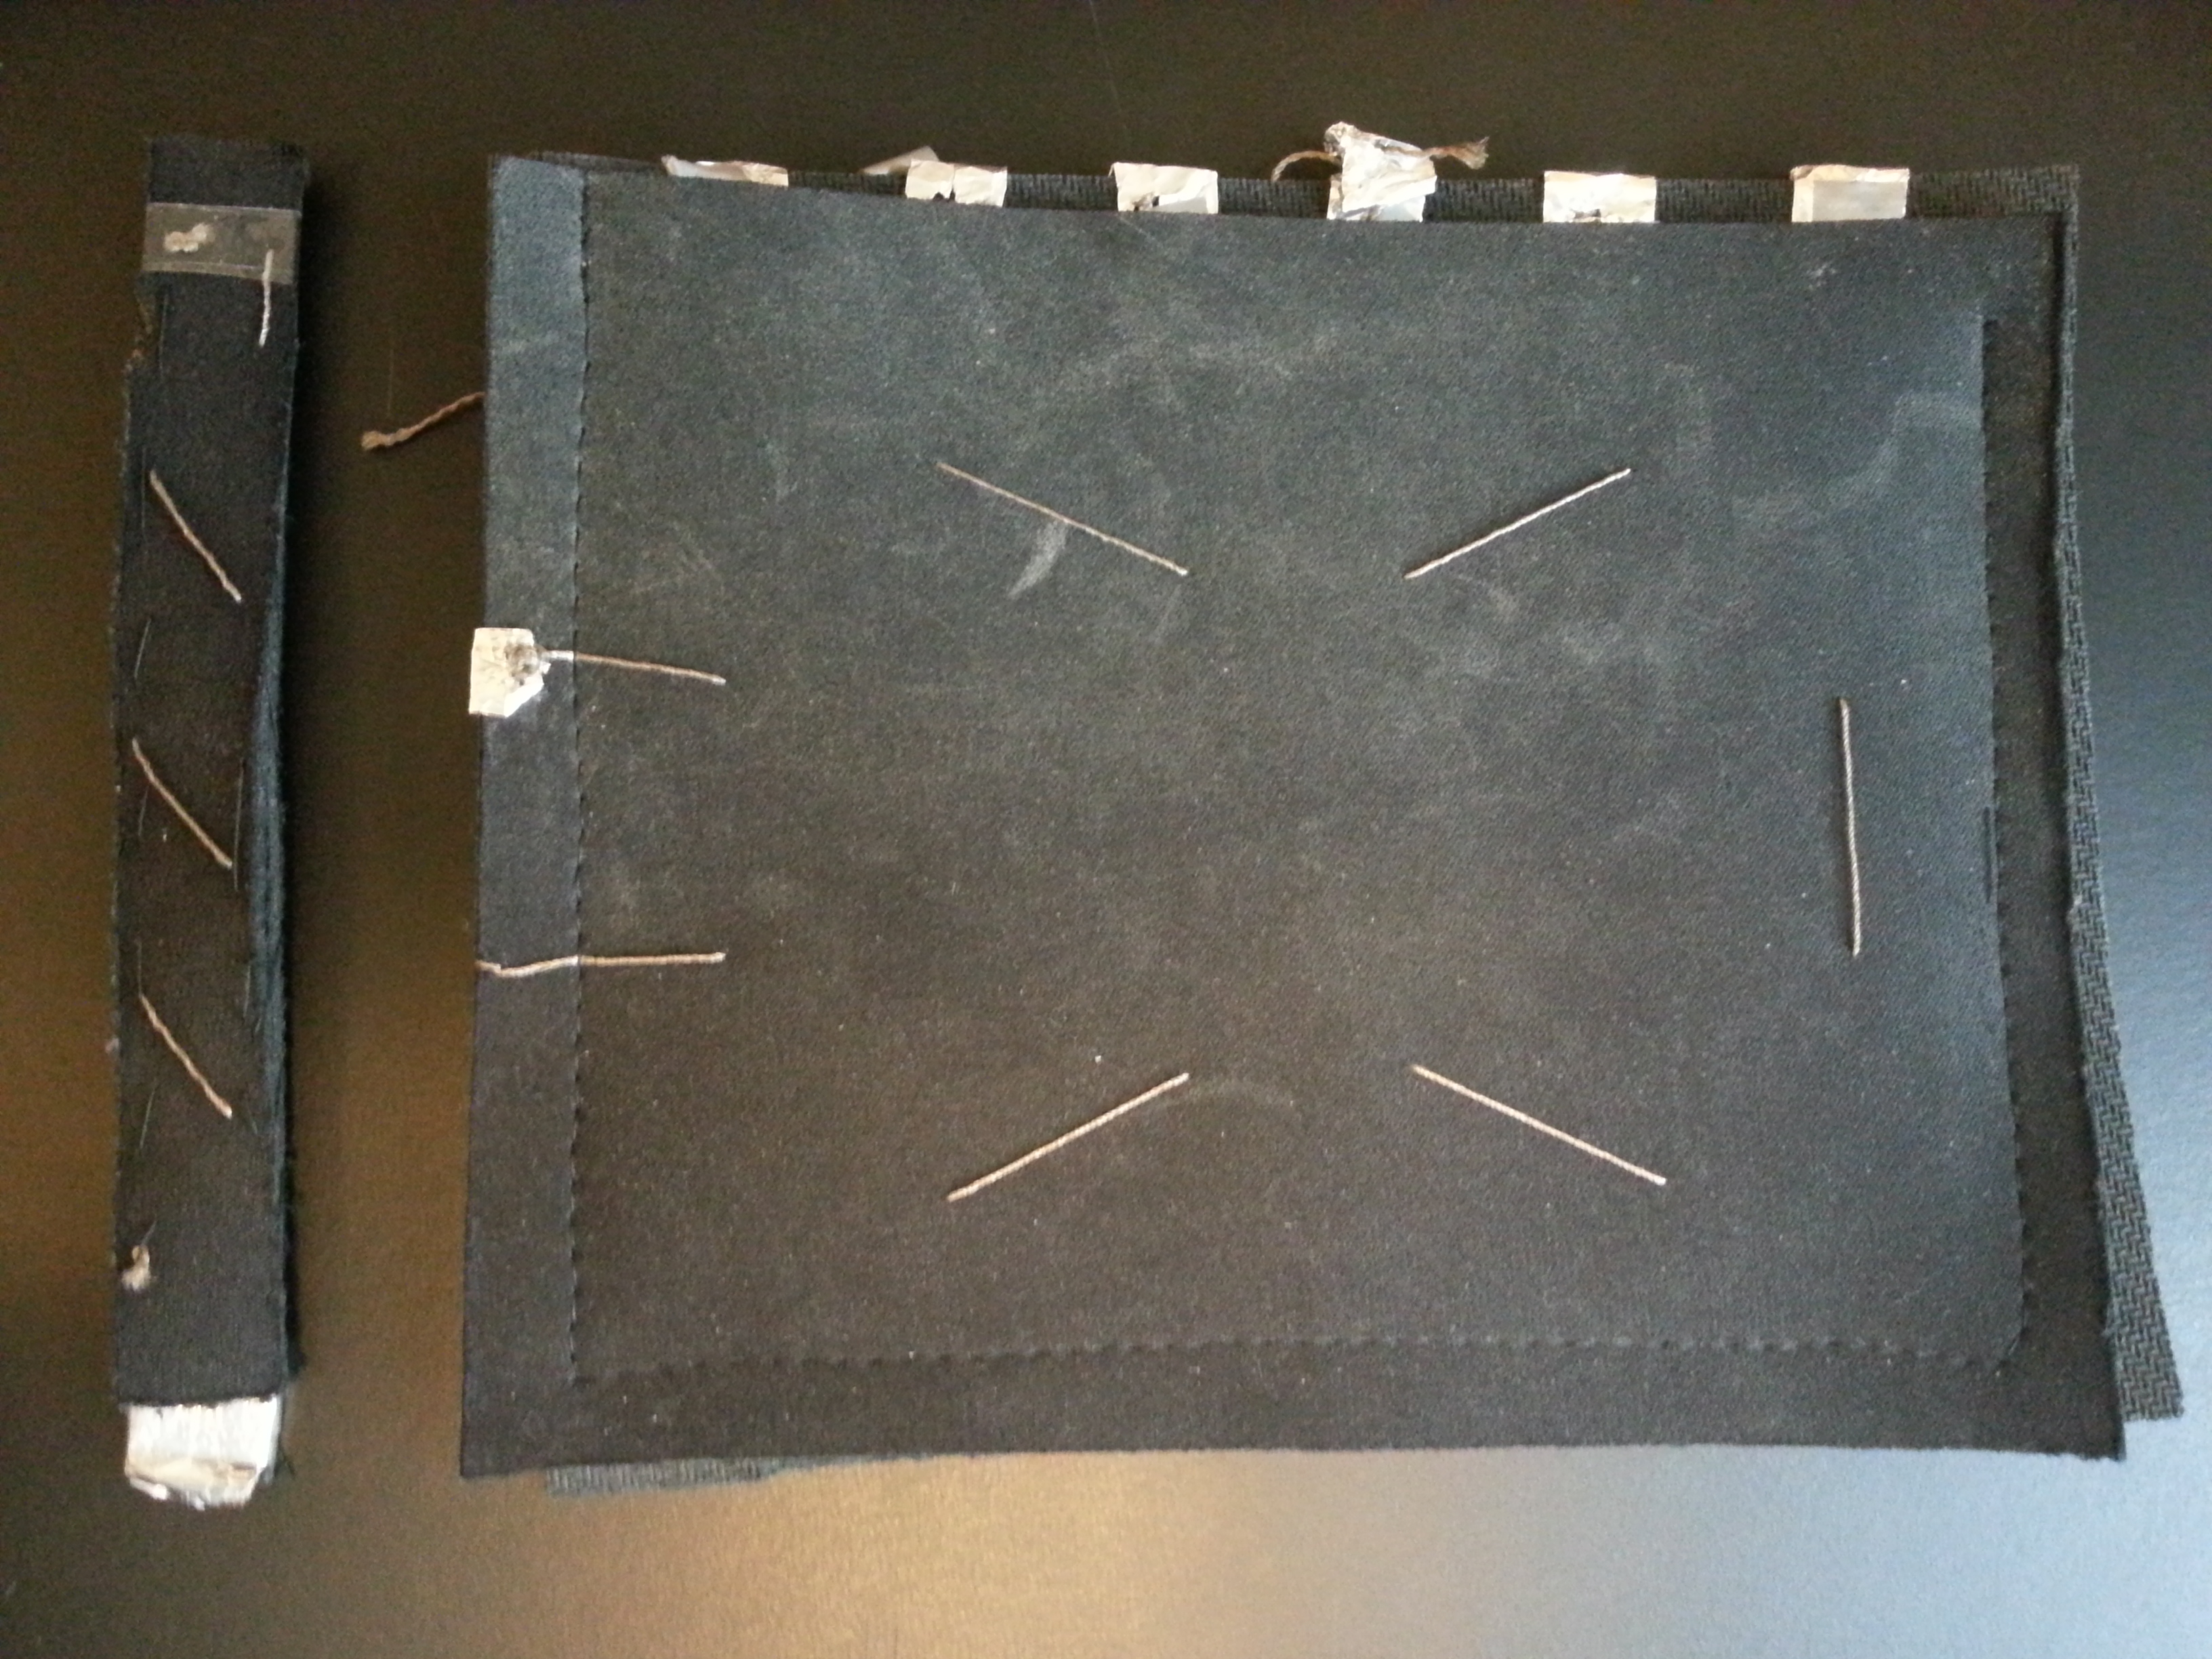
\includegraphics[width=.9\linewidth]{figures/touch/proto1_1}
  \caption{On the left is our simple bend sensor and on the right our 2x3 pressure matrix.}
\end{subfigure}%
\begin{subfigure}[t]{.5\textwidth}
  \centering
  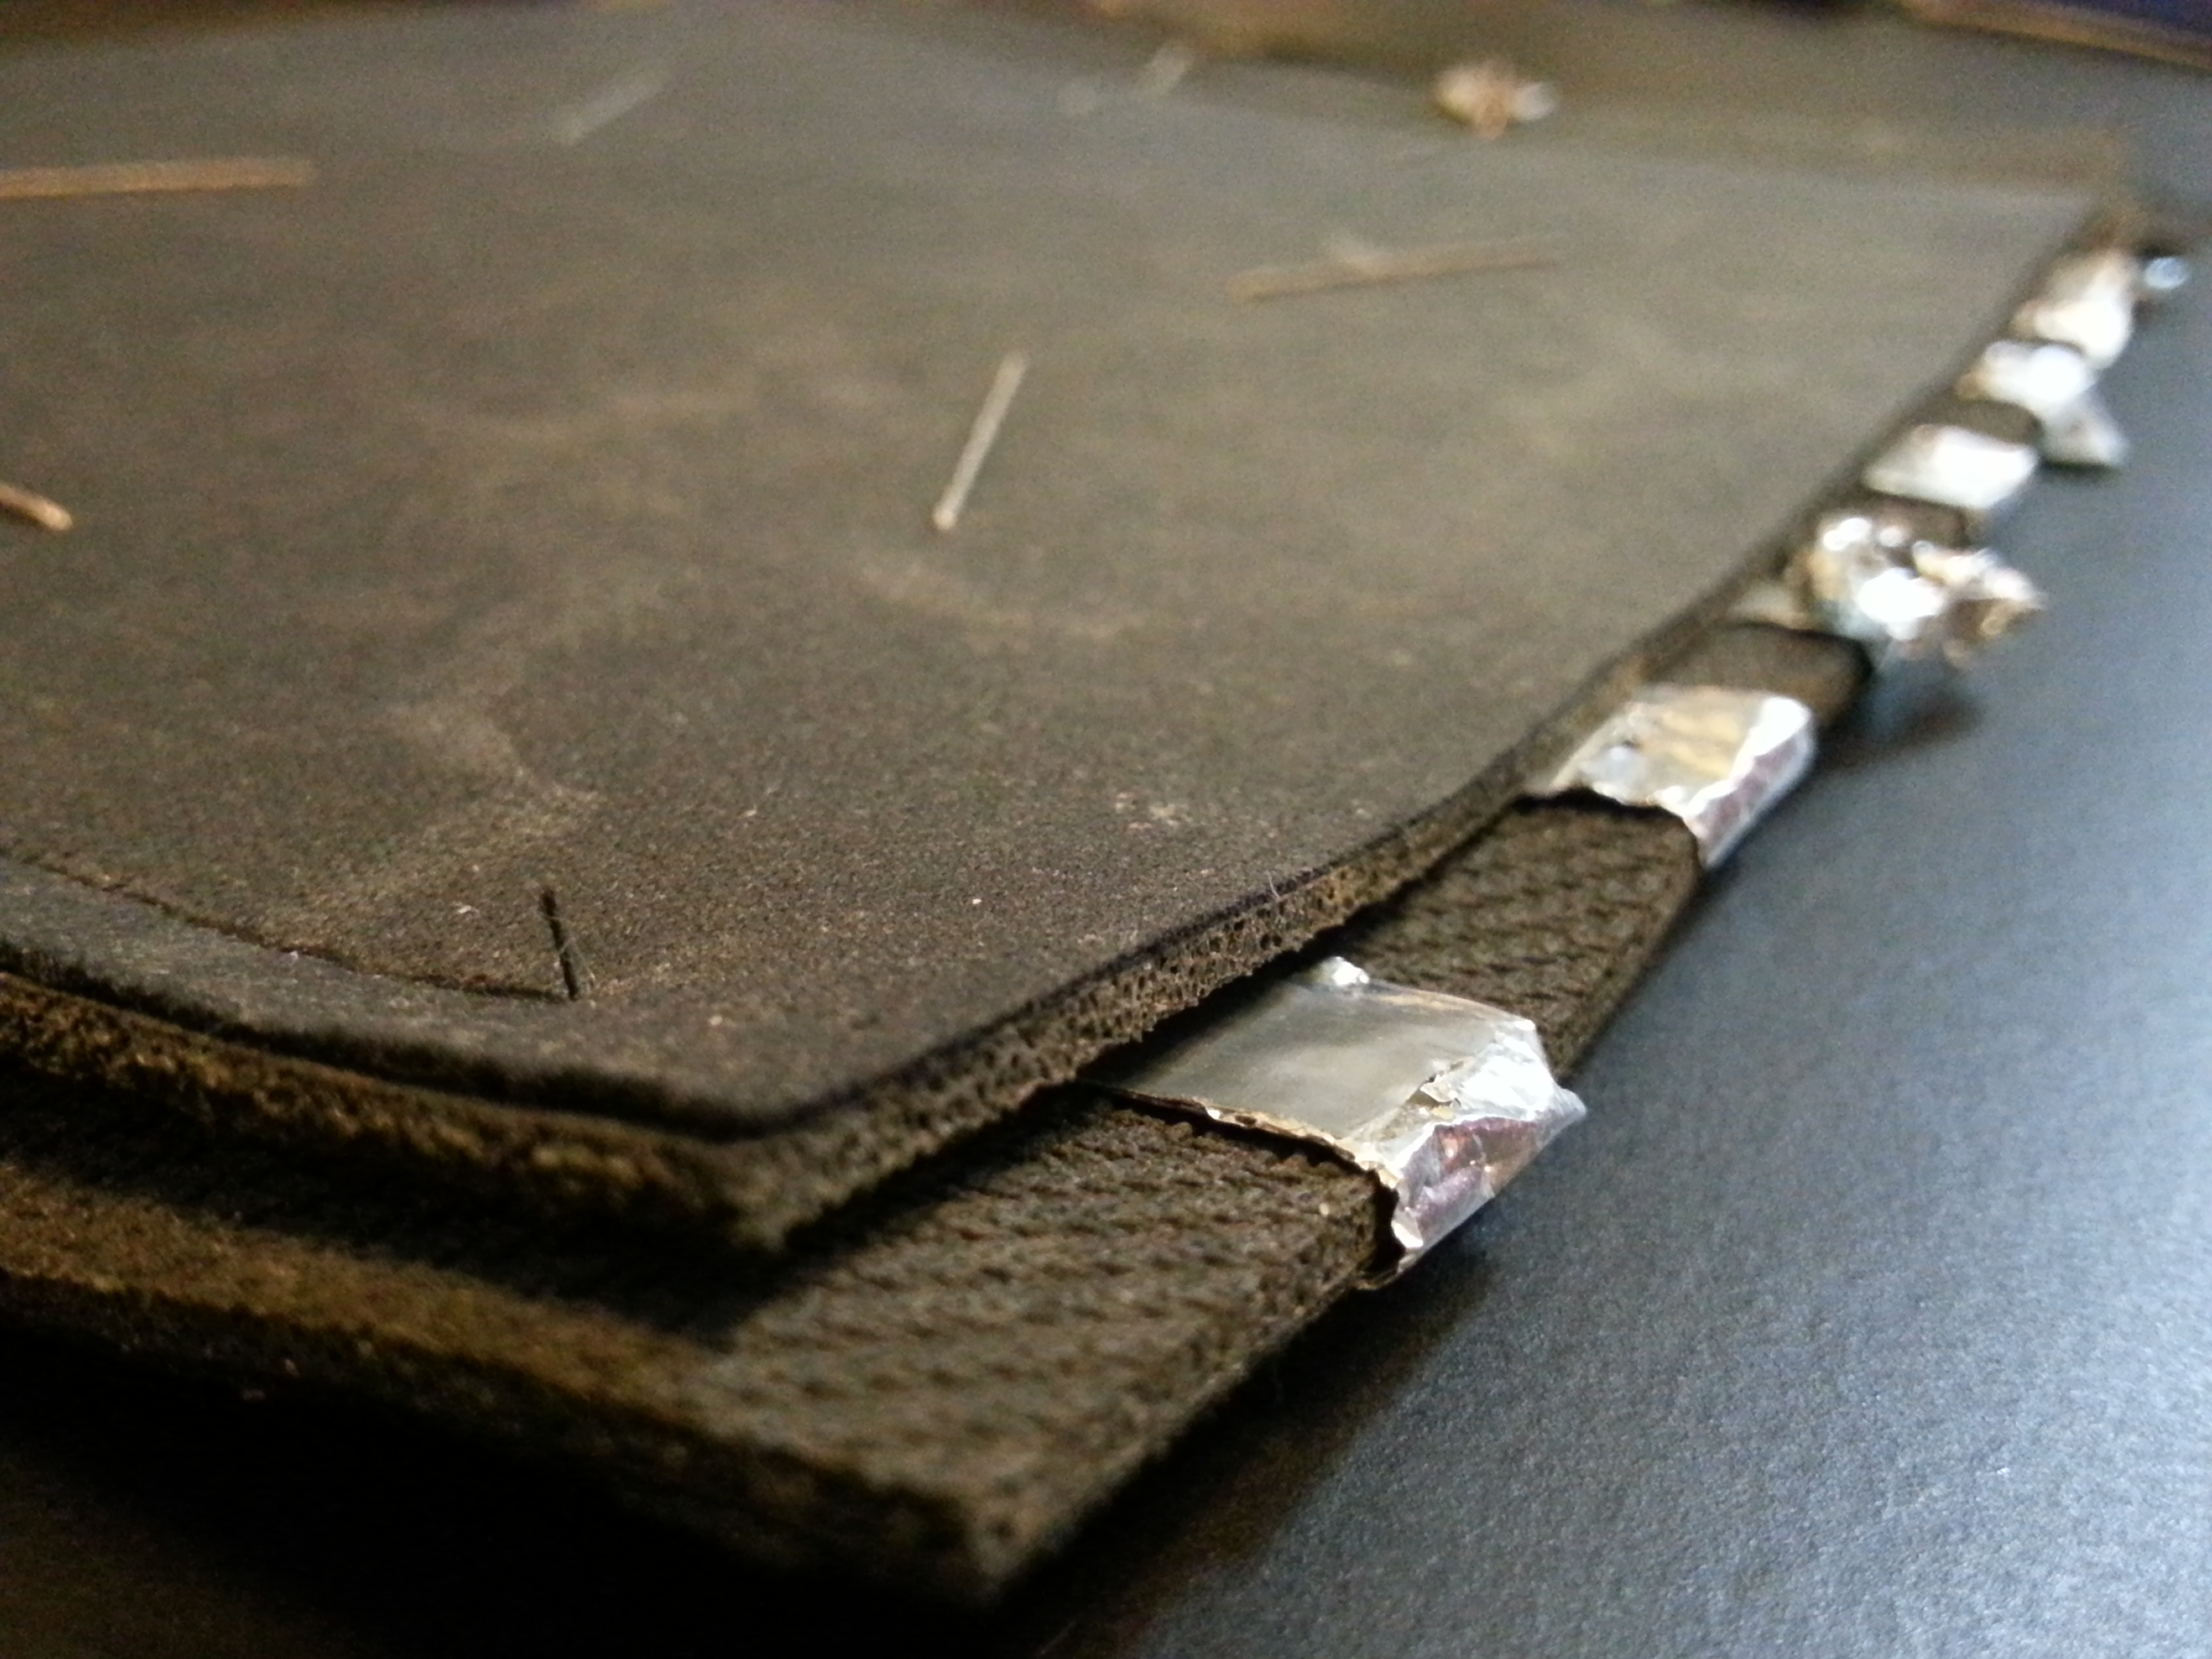
\includegraphics[width=.9\linewidth]{figures/touch/proto1_2}
  \caption{A close up of the materials.}
\end{subfigure}
\caption{First iteration of our touch prototype}
\label{prototype_1}
\end{figure}

By sending a 5V signal into the single top layer stitch, each of the six (\(2*3\)) bottom layer outputs can now be read on the Arduino after passing through the piezoresistive material.  
As pressure is applied to the different sections the voltage drop at the individual grid locations can now be measured with the analog input pins on the Arduino.
The ADC on the Arduino then translates the measured voltage, between 0--5V, into the amount of pressure that is applied to each of the cells, as a number between 0--1023.
The measured numbers will never reach the extremes as there is always some amount of resistance in the material.
A single layer of our anti-static bags have resistance values from around 180-200 KOhms, with little to no pressure applied, down to around 1.8 kOhms when pressed hard.
Depending on the piezoresistive material and the construction of the sensor, these values will vary, \citep{rosenberg2009unmousepad} reports values between 1.2 MOhms and 2.2 kOhms for their FSR ink.

\begin{figure}[h]
	\centering
  		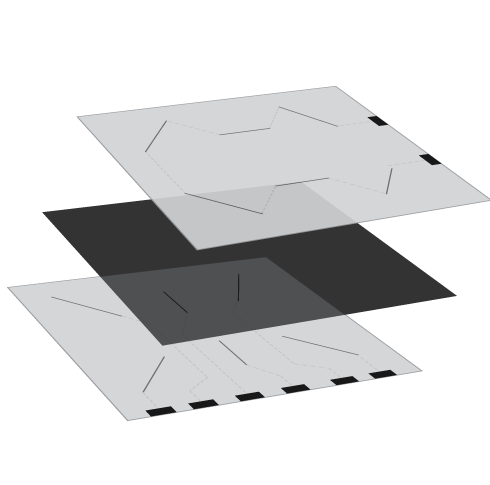
\includegraphics[width=3in]{figures/touch/layers_it_1}
	\caption[The three layers of our touch sensitive fabric, iteration 1.]
   {The three layers of our touch sensitive fabric showing the construction principle of iteration 1.}
   \label{layers_iteration1}
\end{figure}

Each of the cells acts in principle as a discrete sensor as they have their own individual output and are not influenced by each other.
This approach is simple, both in terms of Arduino setup and coding, and can attain the fastest possible update rates as no computation is needed to determine the location of the touch. 
The data received from the sensors is sent to Processing for visualization as can be seen in figure~\todo{ref} which we have used for testing.

\subsubsection{Conclusion}
This quite simple prototype showed us that the basic principles for constructing a textile touch surface with the materials we have had access to, is indeed possible.
One of the major obstacles we found though was the transition from soft electronics (thread and anti-static bags) to hard electronics, as the conductive metal in the threads are woven into normal cotton thread, making soldering extremely hard.
For this first iteration we made due with glued on tin foil connectors as a quick-and-dirty solution.

A major downsides to making touch surfaces as a grid of discrete sensors, as we did in this iteration, is the lack scalability.
There has to be an input pin for each cell in the touch grid you create, so for a given number of rows \(i\) and columns \(j\) you need hardware I/O pins equal to \(i*j\), which is not a suitable for normal micro-controllers which usually have 10--20 I/O pins.
So with this approach we would, just barely, be able to make a 4 x 4 grid with our Arduino Uno. 

\subsection{Iteration 2}
\label{ch:textiletouch:it2}
To combat the lack of scalability in iteration 1 we build a new version of the prototype.
To increase our touch surface resolution we improved the prototype in two ways, first by an improved construction and sewing approach inspired by rSkin \citep{rSsininstructables,rskinplusea} and secondly with interpolating post-processing of the input data inspired by \citep{rosenberg2009unmousepad}. 

\subsubsection{Construction principles}
For the second iteration we made a new 7 x 7 grid prototype, as seen in figure~\ref{prototype_2}, and instead of neoprene, we used sofa textile to get a more natural look and feel, and a larger degree of flexibility in the material.
We used the same basic three layer principle from iteration 1, but in order to solve the scalability issue the conductive thread is sewn in rows and columns as illustrated in figure~\ref{layers_iteration2_and_3}.
The principle is to first activate row 0, then read the output on each of the columns, then activate row 1 and read output on all columns, and so on, contentiously scanning the grid one row/column at a time.
To reduce the sensor noise non active rows and columns are connected to ground throughout the sweep.
Each finished sweep outputs a pressure map that is sent to our applications.

\begin{figure}[h]
	\centering
  		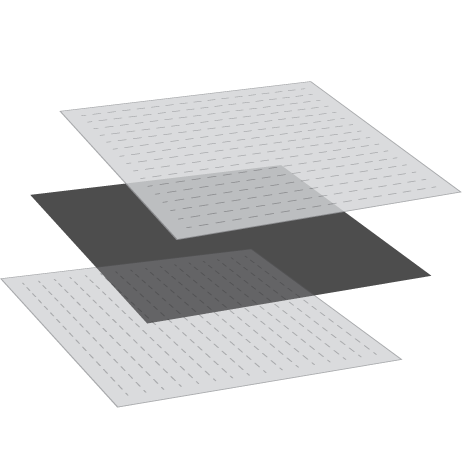
\includegraphics[width=3in]{figures/touch/layers_it_23}
	\caption[The three layers of our touch sensitive fabric, iteration 2 and 3.]
   {The three layers of our touch sensitive fabric showing the construction principle of iteration 2 and 3.}
   \label{layers_iteration2_and_3}
\end{figure}

As only one row and one column are active at a given time the micro-controller now only needs to have one I/O pin for input and one for output and can instead rely on multiplexers\footnote{http://en.wikipedia.org/wiki/Multiplexer} to shift the currently active row/column.
As a result the number of I/O pins now needed is dependent on the number of multiplexers that are used, greatly reducing the number needed for larger grids.

Generally for a multiplexer with \(2^n\) inputs, n control pins are needed plus one pin for the actual signal.
So for a \emph{j} x \emph{i} grid, the amount of pins needed would be \(\sqrt{j*i}\), compared to the \(i*j\) from iteration 1, reducing the amount of I/Os needed by the square root.

As mentioned earlier, if pressure is applied to the piezoresistive material the resistance decreases.
So if the fabric is bend or deformed in any way, this will happen, as the deformation puts stress on the material.
To allow the fabric to be bendable while attaining sensitivity we added a function to `reset' the pressure map by taking a snapshot of the pressure map in its bended state and use this snapshot to subtract from the outputted pressure map.

\begin{figure}[h]
\centering
\begin{subfigure}[t]{.5\textwidth}
  \centering
  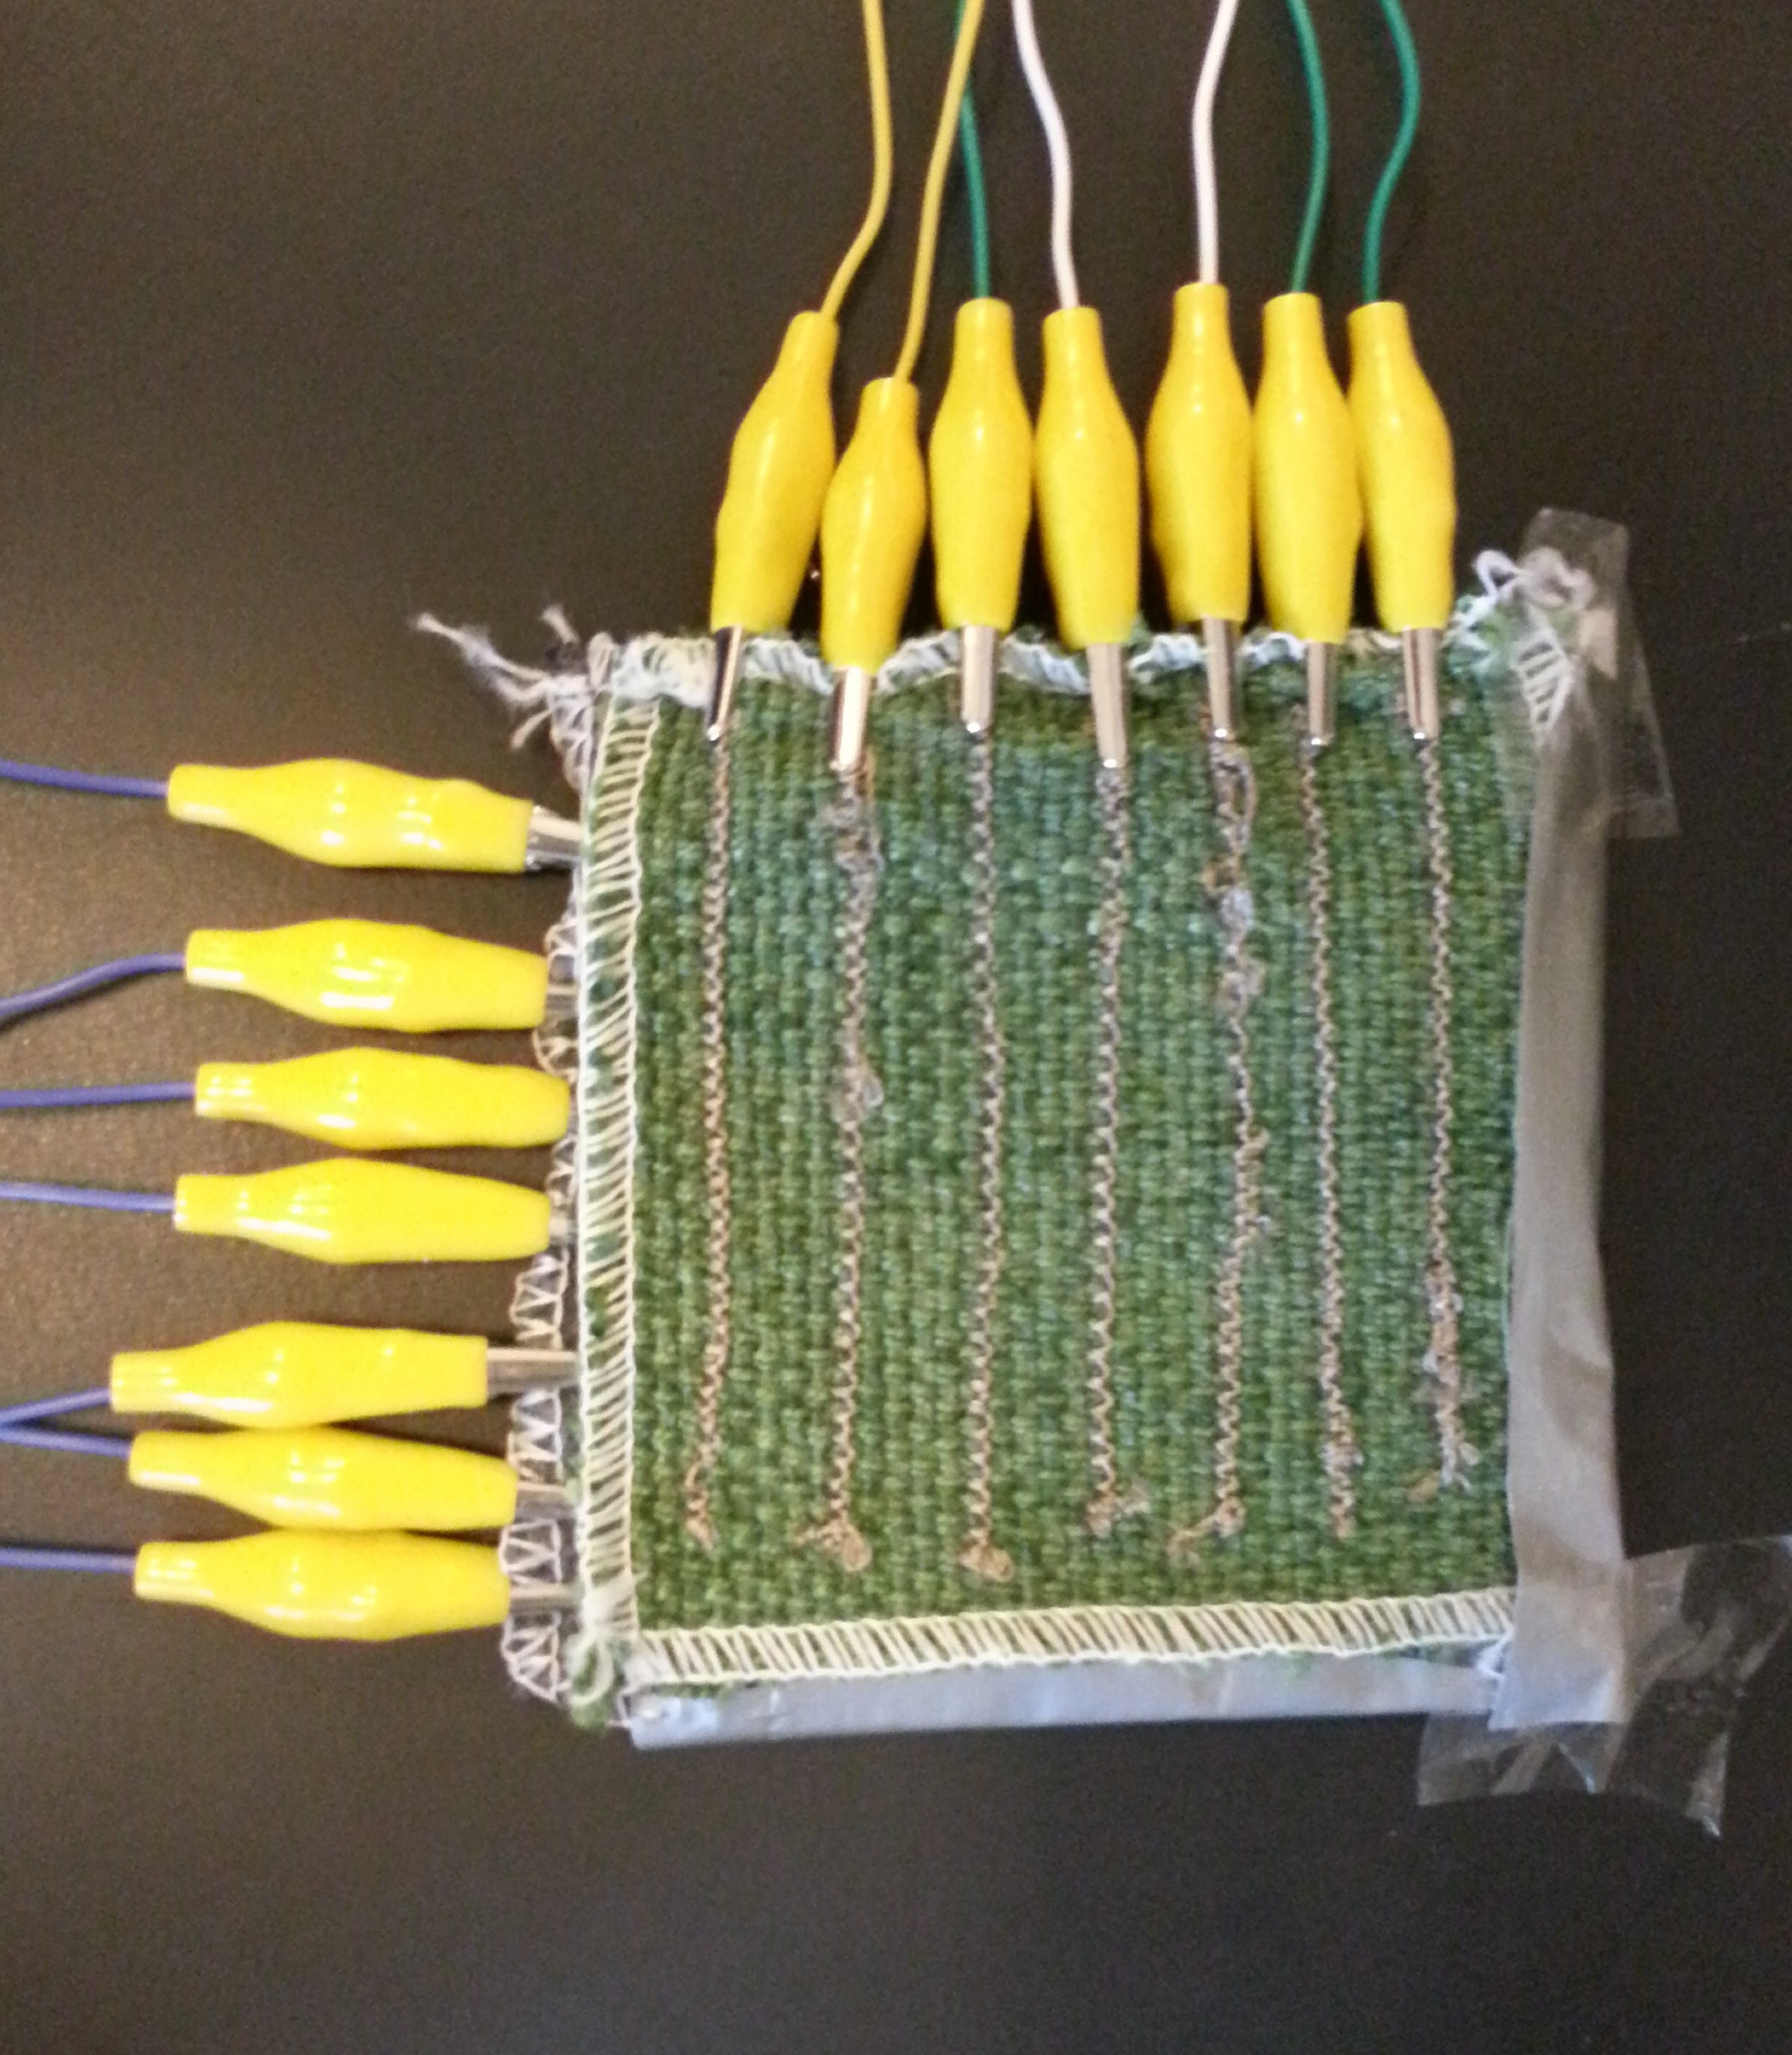
\includegraphics[width=.9\linewidth]{figures/touch/proto2_1}
\end{subfigure}%
\begin{subfigure}[t]{.5\textwidth}
  \centering
  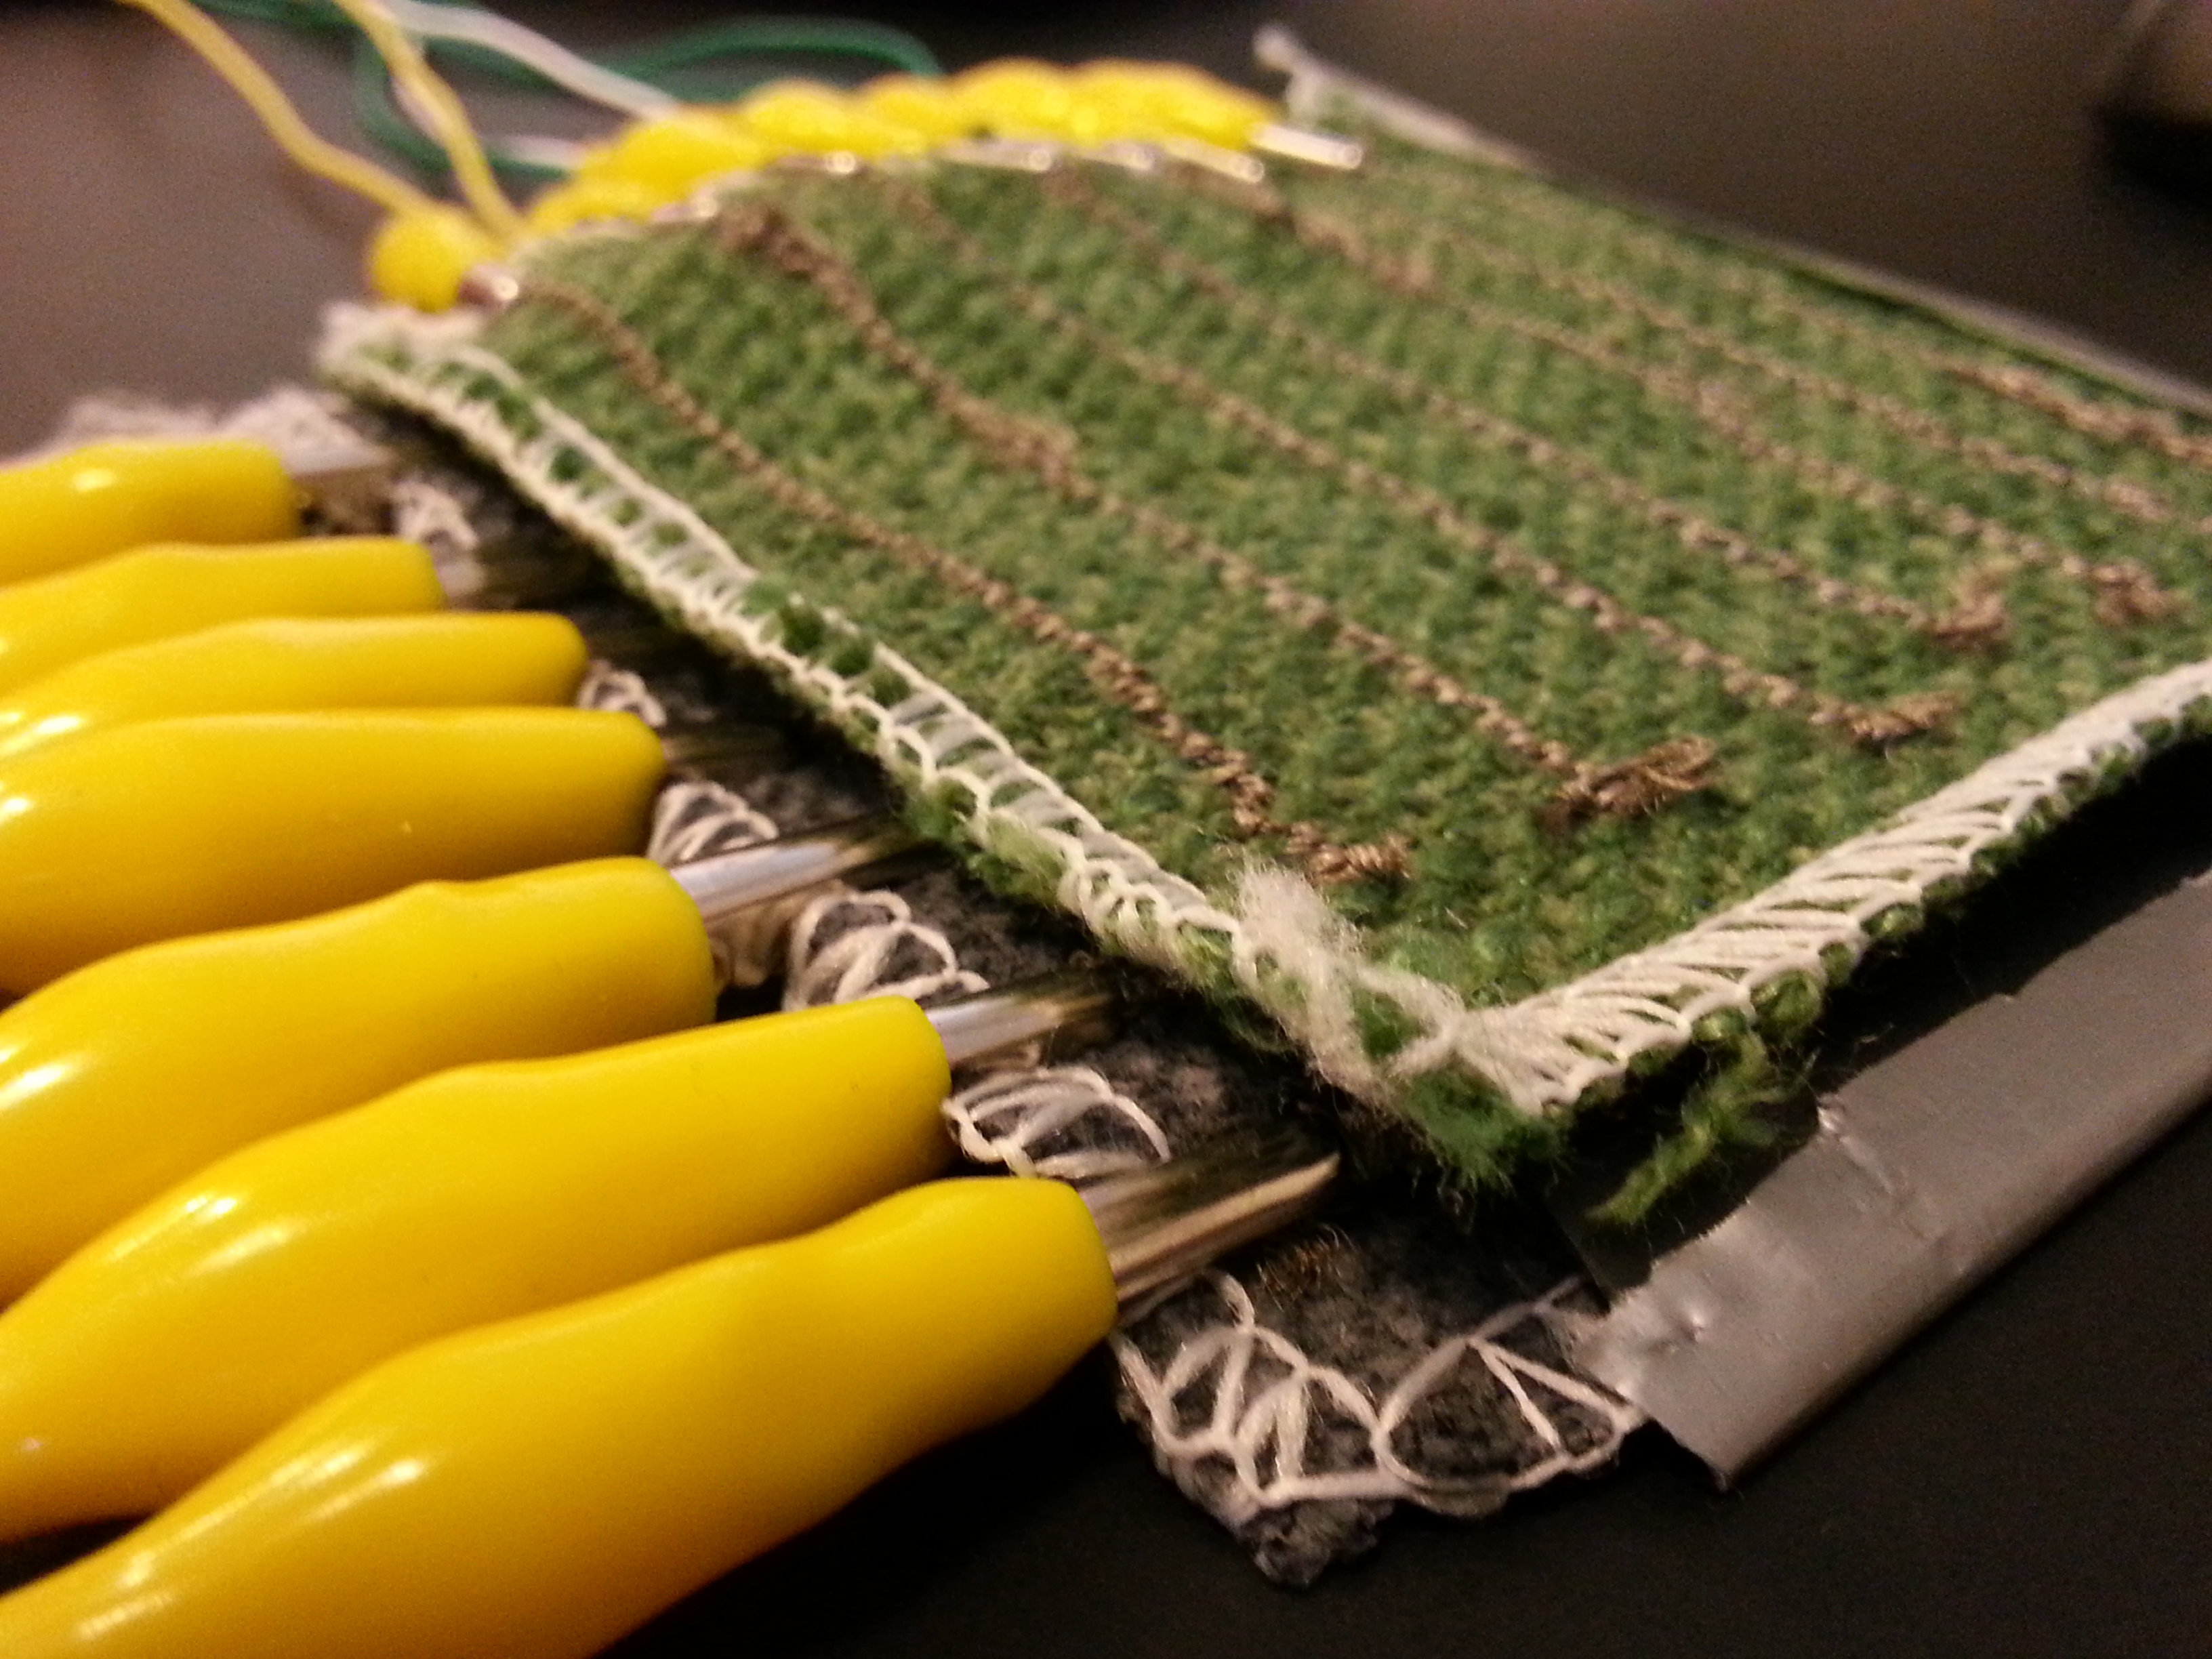
\includegraphics[width=.9\linewidth]{figures/touch/proto2_2}
\end{subfigure}
\caption{Second iteration of the prototype. The interactive area is a 7 x 7 grid with each row and column spaced approximately 1 cm apart from each other.}
\label{prototype_2}
\end{figure}

We now have a 7 x 7 grid fabric pad which in it self gives us a resolution of 49 cells compared to the 6 from iteration 1.
To increase this even further we now go from hardware to software.

\subsubsection{Peak detection and interpolating FSR}
\label{ch:textiletouch:it2-ifsr}
If a touch is made between two rows or columns or current approach will register the touch at the closest row/column intersection instead of the true position.
To improve on this aspect, \citet{rosenberg2009unmousepad} presents a new approach to making FRS sensors called IFSR, or Interpolating Force Sensitive Resistance, in their UnMousePad project. The basic principle is to utilize that each sensor cell has overlapping regions of sensitivity with its neighbours.
This overlapping sensitivity is due to the fact that pressure at some position would also affect the surrounding neighbours as they are connected though the resistive middle layer.
This causes a spatial drop-off in sensitivity at the surrounding neighbours that is near linear for both the X and Y axis.
The fact that it is linear on both axes allows for bilinear interpolation to determine the location of touches between the conductive row/column lines, effectively increasing the resolution. 

Compared to the UnMousePad, which uses printed conductors, our fabric approach is a lot less `perfect' in its construction precision.
At the same time the fabric can bend and twist a lot more that a sheet of polymer, all in all generating a less precise pressure map which translates into less precise interpolation.
As a result we have taken a slightly more simple approach to the interpolation than \citep{rosenberg2009unmousepad} and in turn sacrificed some of the possible resolution gain.
\blank
For a given touch we first find the max value of the nearest intersection of the touch, point \(P_{max}\).
Because a touch gives a radial spread of current around itself, the precise location of the touch will always be in the region of the \(P_{max}\).
As there is a linear drop-off we can now take the readings from the surrounding \((X_{max}\pm1,Y_{max}\pm1))\) and use them them to do a weighted average on both axes to approximate the correct position.
The new approximated point \(P_{approx}\) will, as a result of the radial spread, have a higher weight than the sensed \(P_{max}\) so we scale the value of \(P_{approx}\) with a factor according to the euclidean distance to \(P_{max}\). 

\todo{maaske lidt mere her}

\todo{lav en af ligning interpolationen?}

\begin{figure}[h]
\centering
\begin{subfigure}[t]{.45\textwidth}
  \centering
  
\includegraphics[width=.9\linewidth]{figures/touch/p_map}
  \caption{Visualization of the raw touch data, black indicate no pressure and white indicate high pressure.}
\end{subfigure}%
\hspace{0.5cm}
\begin{subfigure}[t]{.45\textwidth}
  \centering
  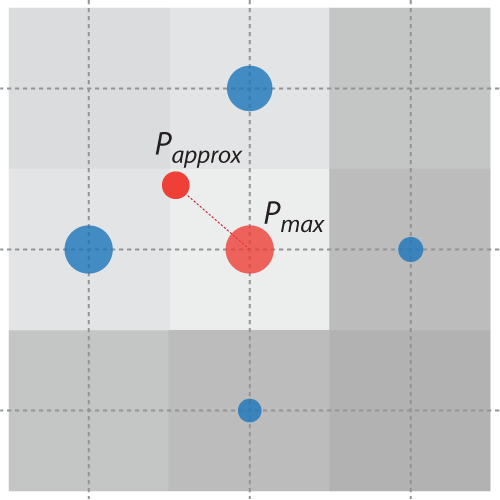
\includegraphics[width=.9\linewidth]{figures/touch/p_approximation}
  \caption{The weight-approximated position, based on the raw touch data from (a). The blue circles indicates the intensity of the values of the sensor cells surrounding the \(P_{max}\).}
\end{subfigure}
\caption{Illustration of the interpolation process.}
\label{interpolation}
\end{figure}

\subsubsection{Conclusion}
For this type of application where a large number of individual sensor cells are needed the construction approach we have used in this iteration is by far superior to the one from iteration 1.
It is a more complex setup both in software and hardware but it does in turn enable much larger sensor arrays than before as we showed before with the amount of I/O pins needed.
As it scales up it is of course more computational heavy on the Arduino CPU as the multiplexers and, in our case, 49 sensor cells needs to be controlled, but as this is still only a 7 x 7 grid we did not experience performance problems.

The interpolation point approximation was, to some degree, a success as it enabled us to up-scale the resolution with a factor 5 with only few approximation errors, but when scaled with a factor 10, which was the goal, quite a few errors appeared.
Many of these errors are due to the sewing of the conductive thread as it, because of the close seams, protrudes a bit where the stitches are, which can be seen by looking at figure~\ref{prototype_2}.
Also the fact that the precision of the sewing are not machine-accurate somewhat eliminates the linearity that we base our interpolation on, creating errors in the raw data that are hard to even out in the software.

\subsection{Iteration 3}
\label{ch:textiletouch:it3}
One of the focus areas of iteration 3 was build a larger and more precise version of iteration 2 as to get more reliable raw data from the sensor grid to use for gesture interaction.
As we were aware of the possibility of generating imprecise data, as we have discussed in the previous iterations, from physical deformation, construction imprecision, material variations and approximation errors, the second focus was to implement a basis for gesture recognition that would function under these constraints.

\subsubsection{Construction Principles}
We used the same setup of iteration 3 but scaled to a 16 x 16 grid, providing 256 sensor cells after software upscaling, compared to the 49 of iteration 1.
The prototype was made in linen which is robust but a lot finer and thinner that the sofa textile and the conductive thread was sewed with less close seams to avoid some of the problems from iteration 2.
The prototype can be seen in figure~\todo{ref} and the schematics for the final hardware setup can be seen in appendix \ref{app:textile-touch}.

One of the main challenges in the construction of this iteration was the attachment of the wires to the conductive thread.
In iteration 1 we tried with glued on tin foil which only worked because we only had 6 connections to handle.
The 14 connections in iteration 2 were connected with alligator clips which, besides not looking elegant, tend to cause deformation of the fabric as they close upon it.
As we now had 32 connections to deal with we found that using ribbon cables would give a better structure.
Furthermore, as alligator clips were out of the question and as tin and textile do not work well together we needed to find an alternative for the connection.
Conductive paint turned out to be a good substitute and worked as a kind ``cold''-soldering method - a secondary feature of the paint.
As the paint dries it functions like an adhesive but with the added ability of being conductive so you avoid the risk of the glue get in between the two conductors severing the connection, see figure~\ref{fig:ch:textiletouch:barepaint}.

\begin{figure}[t]
\centering
\begin{subfigure}[t]{.45\textwidth}
  \centering
  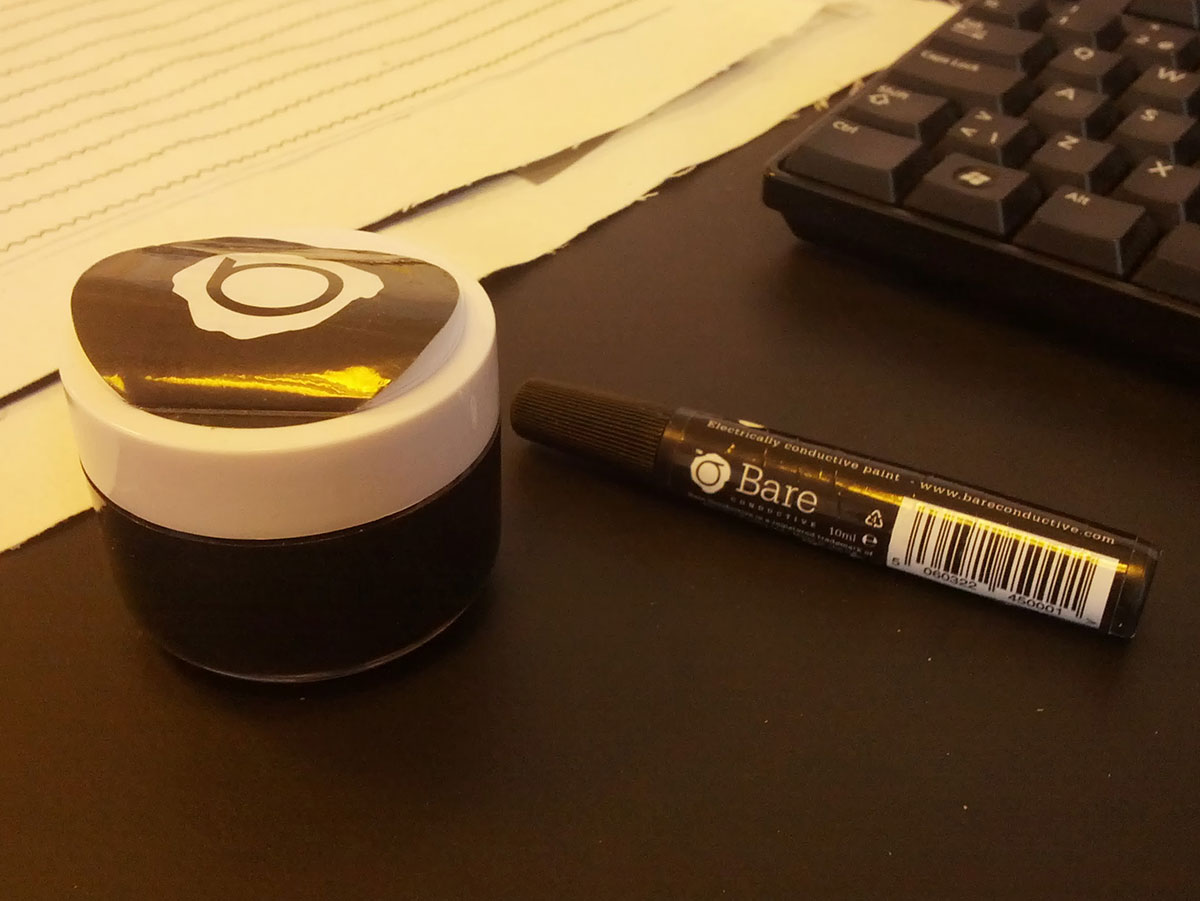
\includegraphics[width=.9\linewidth]{figures/touch/barepaint}
  \caption{Bare Paint, an electrically conductive ink, found at www.bareconductive.com}
\end{subfigure}%
\hspace{0.5cm}
\begin{subfigure}[t]{.45\textwidth}
  \centering
  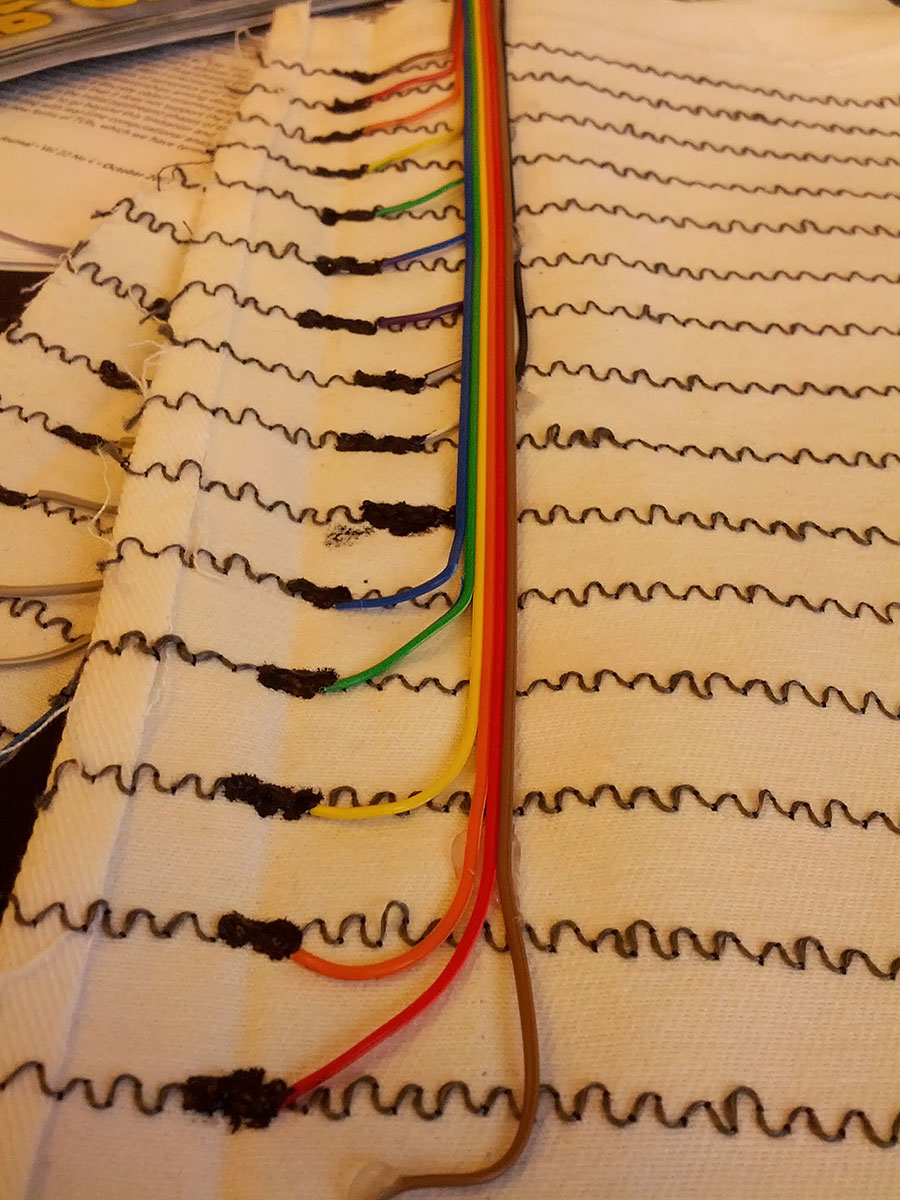
\includegraphics[width=.9\linewidth]{figures/touch/connectors}
  \caption{Bare Paint, used for ``cold''-soldering wires to conductive thread.}
\end{subfigure}
\caption{One solution for the challenge of connecting conductive thread to wires.}
\label{fig:ch:textiletouch:barepaint}
\end{figure}

\subsubsection{Data flow}
In figure~\ref{fig:textiletouch:dataflow} we illustrate each major step in the data flow and processing 
of our prototype.
The flow of data starts from sensor data in the \emph{physical layer} read by the Arduino.
Thereafter it is converted to digital data and streamed to the \emph{processing layer}.
In the \emph{processing layer} the data goes through several filter stages to optimise the data.
Lastly the filtered data is delivered to \emph{application layer} where data can be translated into gestures or visualisations.
We have already covered the principles of the physical layer in \ref{ch:textiletouch:it1} and peak detection and interpolation in \ref{ch:textiletouch:it2}.
Next we will cover some additional steps in the data flow and the \emph{application layer}.

\begin{figure}[b]
  \centering
      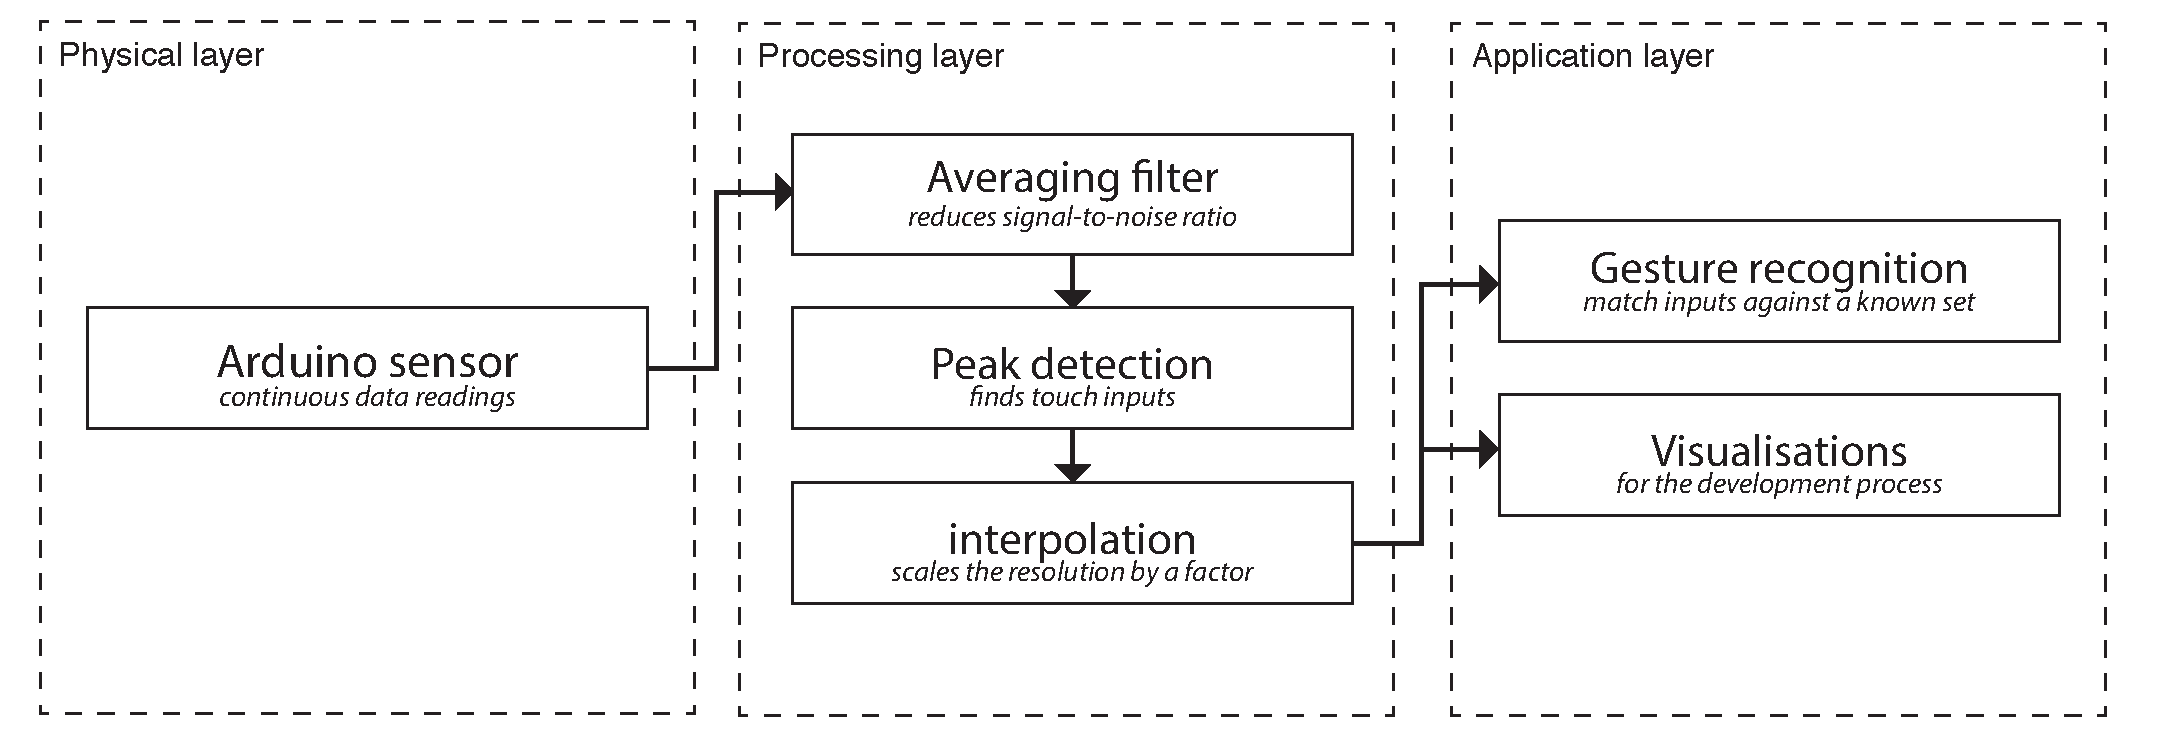
\includegraphics[width=\textwidth]{figures/touch/dataflow}
  \caption[The data flow from sensor to application.]
   {Textile Touch data flow from sensor to application.}
   \label{fig:textiletouch:dataflow}
\end{figure}

\subsubsection{Noise reduction}
On the software side we have implemented a simple averaging filter to reduce noise by increasing the signal-to-noise ratio, SNR.
This filter takes each input frame and averages the values of each cell with the cell values of \(x\) previous frames.
We have found that averaging over the past \(x = 2\) frames gives the best result for our setup. 
\todo{udpensles mere?} 
In this way noise such as sudden spikes will be reduced while preserving the actual touch values of the frame.

\subsubsection{Peak detection and interpolation}
The algorithm for detecting touch input and interpolation has generally not changed since iteration 2, see~\nameref{ch:textiletouch:it2-ifsr} in \ref{ch:textiletouch:it2-ifsr}.

The new part is that we in iteration 3 also have introduced multi-touch input.
This is more a proof of concept feature which will not be fully functional and stable for interaction. The reason for this is that our code needs some adjustments to be able to provide proper stroke data to the recognition framework which would require too much implementation time.
So for now we can visualise multi-touch input and basically use it for drawing, see figure~\ref{fig:textiletouch:multitouch}.

An alternative would be to serve all recorded touch points to the \$N implementation, as opposed to \$P, \todo{but as noted earlier} this would be unsatisfactory slow.

\begin{figure}[h]
  \centering
      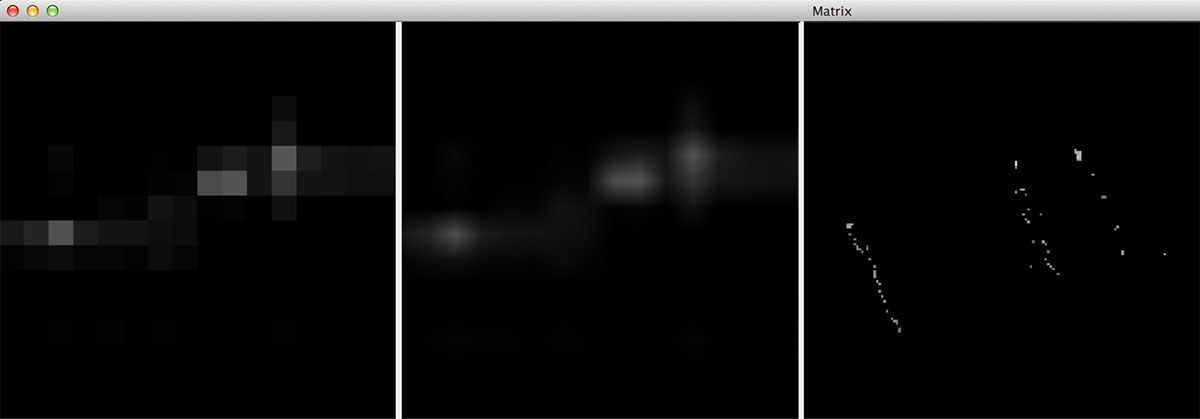
\includegraphics[width=.9\textwidth]{figures/touch/tt_multitouch}
  \caption[The data flow from sensor to application.]
   {Multi-touch input visualised. 3 fingers are detected and 3 lines are drawn simultaneously.}
   \label{fig:textiletouch:multitouch}
\end{figure}

\subsubsection{Gesture recognition} 
\label{ch:textiletouch:gesture_implementation}

We have created an application that takes the filtered data of the \emph{processing layer} and abstracts it to a collection of strokes that are delivered to the \$P gesture recognition framework, which matches the input up against a set of predefined gestures templates.
The dollar family of recognizers were presented earlier in \ref{ch:textiletouch:gesture_recognition}.
Initially we experimented with the \$N implementation which was able to recognise gestures but with some limitations.

First of all, the recogniser was sensitive to the ordering of the strokes which meant that the it could fail on the same gesture if drawn from different starting points. \todo{Tore, yes?}

Secondly, there was a considerable amount of delay before a resulting gesture was found.
We measured this to be in the area of \(800\) to \(1000 ms\), a latency which in our opinion does influence the user experience.
After changing to the \$P implementation we got this delay down to \(< 10 ms\) which is quite an improvement.
This is because \$P avoids a combinatorial overhead of \$N where \$N matches up against every possible combination of stroke order and direction.

Furthermore, the \$P implementation does not distinguish the order of the strokes which allows for subjective ways of drawing specific shapes.

One limitation of both implementations is that they do not take in to account the orientation of the input. 
This means that, for example, for a line to be recognised in both a vertical, horizontal and diagonal version they all need to have a predefined template. \todo{say something about the complexity of writing templates? P vs N}

\subsubsection{Feedback} 

\subsubsection{Conclusion} 

Although the 3rd iteration overcame some of the limitations of the 2nd iteration it still has some constraints that we would like to address.

One noticeable limitation is performance as foreseen in interation 2.
Our current Ardiuno Uno is not fast enough to always follow along with quick touch movements on the prototype.
Simple gestures like lines or simple characters are not affected as much as more complicated symbols.
The new and exceedingly faster Arduino Due\footnote{http://arduino.cc/en/Main/ArduinoBoardDue}, an ARM-based board which operates at a clock speed of 84 MHz, has recently been released and would greatly outperform our older 8 MHz Arduino Uno.

One of the reasons for scaling up the prototype was to get a larger area for touch input.
In the process of tripling the dimensions of the prototype (from approximately \(8x8cm\) to \(25x25cm\)) we also increased the amount of rows and columns but with a little extra spacing (\(1.5cm\)) between the individual lines.
It seems that this spacing has become a bit too large, meaning that pressing in between the intersections of two rows and two columns does not propagate quite enough pressure to the surrounding line crossings, resulting in smaller pressure values (see figure~\ref{fig:textiletouch:intersections}).

We have tried to improve this in our approximation algorithm by multiplying the value with a factor relative to distance away from the line in both axes.
This has to some degree amended the issue but not fully.

\begin{figure}
\centering
\begin{minipage}[t]{.45\textwidth}
  \centering
  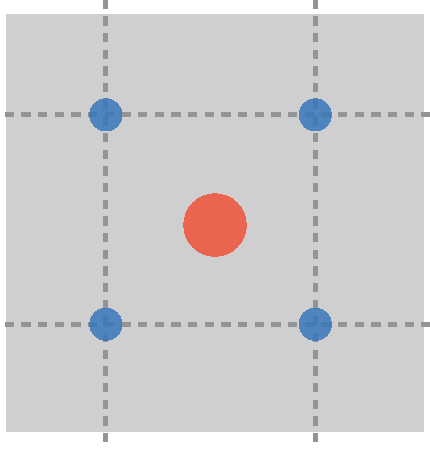
\includegraphics[width=.9\linewidth]{figures/touch/intersections}
  \caption[Pressing in between the intersection of two rows and two columns does not propagate enough pressure.]
  {Pressing in between the intersections of two rows and two columns (red dot) does not propagate enough pressure to the surrounding lines crossings (blue dots).}
  \label{fig:textiletouch:intersections}
\end{minipage}%
\hspace{1cm}
\begin{minipage}[t]{.45\textwidth}
  \centering
  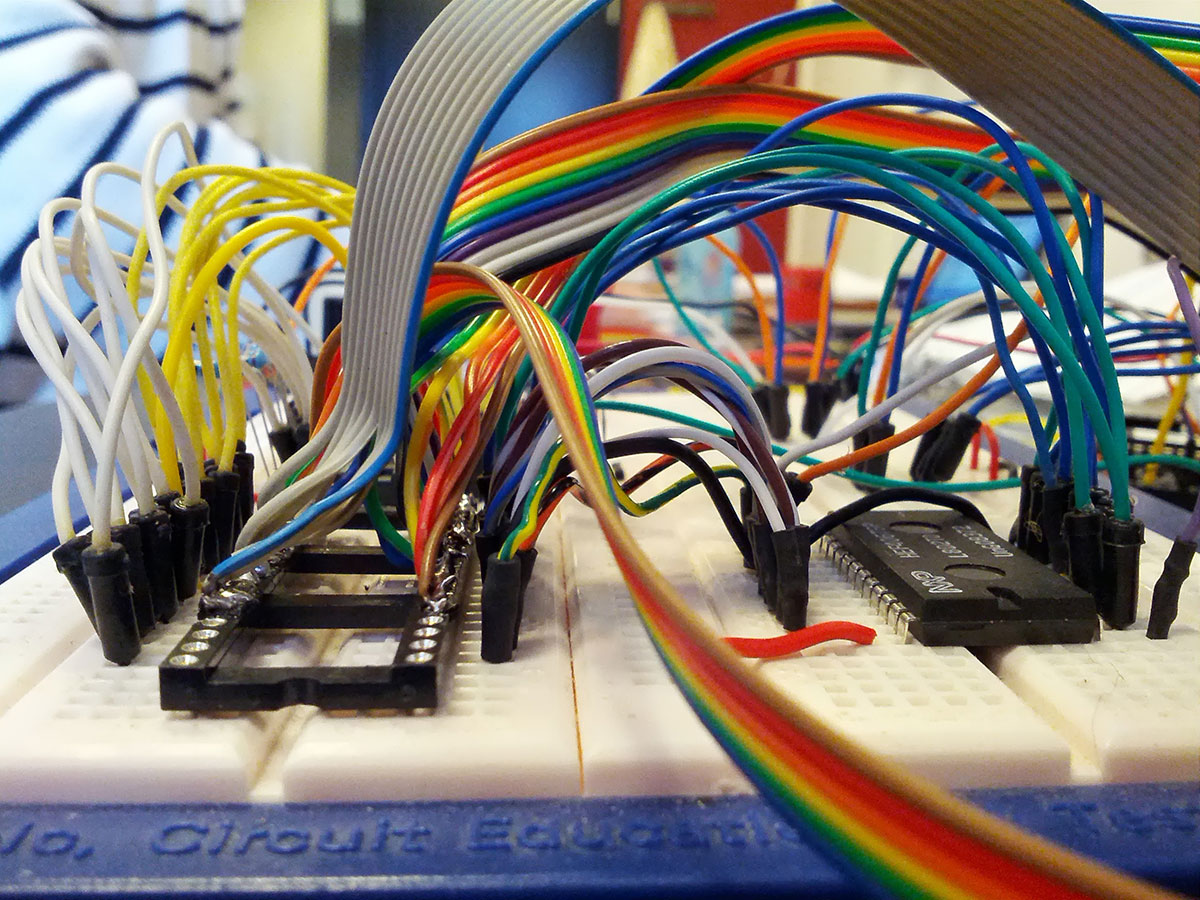
\includegraphics[width=.9\linewidth]{figures/touch/wires}
  \caption[Breadboard crowded with wires.]
  {Breadboard crowded with wires.}
  \label{fig:textiletouch:wires}
\end{minipage}
\end{figure}

An alternative approach is to reduce the spacing again to \(1cm\) or less but that would require quite a few extra wires which we already have quite a few of (see figure~\ref{fig:textiletouch:wires}).
Furthermore increasing the grid resolution would result in an exponential growth in the amount of data to be transmitted by the microcontroller.
With a \(16x16\) grid we are sending 256 values every frame (\(10ms\)),
If we were to lower the spacing to \(1cm\) we would get a grid resolution of \(24x24\) which in turn would require a transmission of 576 values for every frame.
As our microcontroller is already running at over capacity this out of the question for now, but by replacing the microcontroller with a more powerful one, as mentioned before, increasing the resolution could become relevant again.
Therefore we see it as a balance between the size of the touch area and the complexity of the hardware setup.

\begin{verbatim}
- Fokus paa kode (gestures,resolution,performance)
- Interpolering muliggoere tryk mellem linjerne, 10x saa hoej oploesning dog udfald 
  og varierende praesision (vis vi har eksperimenteret med forskellige oploesninger)
- Forskellige visualiseringer til performance evaluering
- Integrering af gesture recognition og test miljoe til dette
- Haptisk feedback, vibration
- Udfordringer: praesision, performance 
  (max baud-rate for hurtigt til at java kunne foelge med)
\end{verbatim}

\section{Evaluation and future work}
%!TEX root = ../thesis.tex
In this section we are going to cover our evaluation of our \emph{textile touch} explorative prototype, more specifically this is the latest prototype covered in \ref{ch:textiletouch:it3}~(\nameref{ch:textiletouch:it3}).
We have two primary goals of this evaluation.
On the one hand, we want to evaluate on the interaction potentials of using simple gestures as input control.
This goal involves using the prototype as an interactive device to control existing devices of the home.
On the other hand, we want to explore our prototype in alternative contexts.
This goal should shed light on the prototypes potential of encouraging alternative usages than controlling existing devices.

Evaluations were done over three rounds to get a diversity in age groups of the test participants and also to evaluate both technical and non-technical people.
\hl{We were interested in shedding light on the diversity of creative ideas a child would bring compared to and adult.
}
\todo{mere + afrunding}
\blank
As mentioned earlier in \emph{ \nameref{ch:textiletouch:it3} } we have developed a simple audio and video application which mimics some of the functionality of a television and a stereo system.
This application was used as the starting point for evaluating the value of using the prototype for controlling existing devices.
During evaluation we would connect the prototype setup and computer to the home TV to resemble the real situation and the prototype would for instance be layn as part a of sofa, as a table cloth or attached to a wall as for example wallpaper.
From there on the basics of interaction were understood and further discussions and explorations could be made extending beyond the limits of the audio/video application.

Moving on from looking at the potentials of controlling existing devices of the home, the evaluations would take a more discussion-oriented direction where alternative usages and activities were the primary focus.
To start off discussions we would present some of our own ideas of potential usages.
\todo{mere}
\blank
An overall note to be taken from the evaluations was that the participants found it intriguing to try out the prototype.
Not so much for the purpose of the simple test application, but more for the idea of interacting with textile and using it for digital input.
Surely they are accustomed to using touch interaction on the small surfaces of everyday consumer devices such as displays and touchpads, but not with inherently non-electronic materials such as textile. \todo{lidt mere generelt her}
\blank
In the next section we will evaluate on the performance of our prototype and then continue on with the conceptual potentials in the subsequent two sections.

\subsection{Performance and feedback}

In this section we will discuss the prototype concerning performance and feedback and some of the improvements suggested during evaluations.

% refresh rate
The limitations of the refresh rate of the hardware were noticed by all participants.
The consequence was that they had to perform touch input in a more careful manner and with slower motions than they wanted to.
The participants' touch strokes were in general much faster than anticipated, which is likely due to us having done much of our testing during development and therefore have been more careful.
They were all able to adapt to it and perform their intended actions with success, but it did of course put a constraint on the interaction.

% softness
In our first evaluation we tested a scenario with a sofa with textile touch embedded.
The softness of the sofa made touch input readings inconsistent and unstable.
The reason for this was that the prototype was not part of the sofa construction which makes even small movements and pressure inputs push the prototype around on the surface of the sofa.
This makes the pattern that constitutes a touch look different than when used on a hard surface which we have not taken into account in our software.

% fb: vibrations
The idea of a pulsating vibration during touch was well received as an indication of touch being recorded and to delimit for example the digital sofa from the physical sofa. \todo{what?}
As we anticipated, the haptic feedback got some critique and it was pointed out that it should give a stronger sensation.
We had placed the vibration motor in the center beneath the prototype and vibrations were therefore only noticeable in that area.
With a less powerful motor the subtle touch sensation of ones hand against the texture of the linen could easily drown the vibrations as well.

% fb: visual on display
A concern brought up by several participants was that there was a lack of indication of the stroke one had just applied.
A promising visual feedback technique for display-oriented interaction was suggested by one of the participants.
The idea was to get real-time feedback on a display when providing touch input by seeing the strokes being made as an overlay on the display.
The strokes would then quickly fade away again to not obstruct the viewing experience. 
In figure~\ref{fig:textiletouch:eval:overlay} we have made an illustration of two semi-transparent strokes overlaying a TV programme as example. 

% fb: visual through LEDS
This visual feedback technique could be very convenient when actions are directed towards a device with a digital display, but not possible in a display-less context.
The single LED we installed beneath the prototype did not prove to be very useful by itself, but its ability to shine through the linen did show potential.
We discussed a larger deployment where a low resolution grid of tiny LEDs could be embedded beneath the textile surface and follow movements by illuminating at touch points and get a direct visual feedback, see figure~\ref{fig:textiletouch:eval:backlighting}.
This approach is again limited to applications where the surface material allows for illumination to shine through, but it does extend beyond textile materials.

\subsection{The concept as a controller for existing devices}
\todo{\dots}
\blank
\begin{verbatim}
taler til det indre dovendyr (paw)
   rette paa gardiner
skal i hvert fald ikke blive et komplekst nyt sprog man skal laere
   ensartet interaktion paa tvaers af applikationer
teenager forstod med det samme - mega smart ;-)
  fandt det let at interagere med
"fjernbetjening er en forlaengelse af min arm" (paw) - dette er dog et lidt vagt modargument
\end{verbatim}

\begin{figure}[h]
  \centering
  \begin{subfigure}[t]{.44\textwidth}
    \centering
    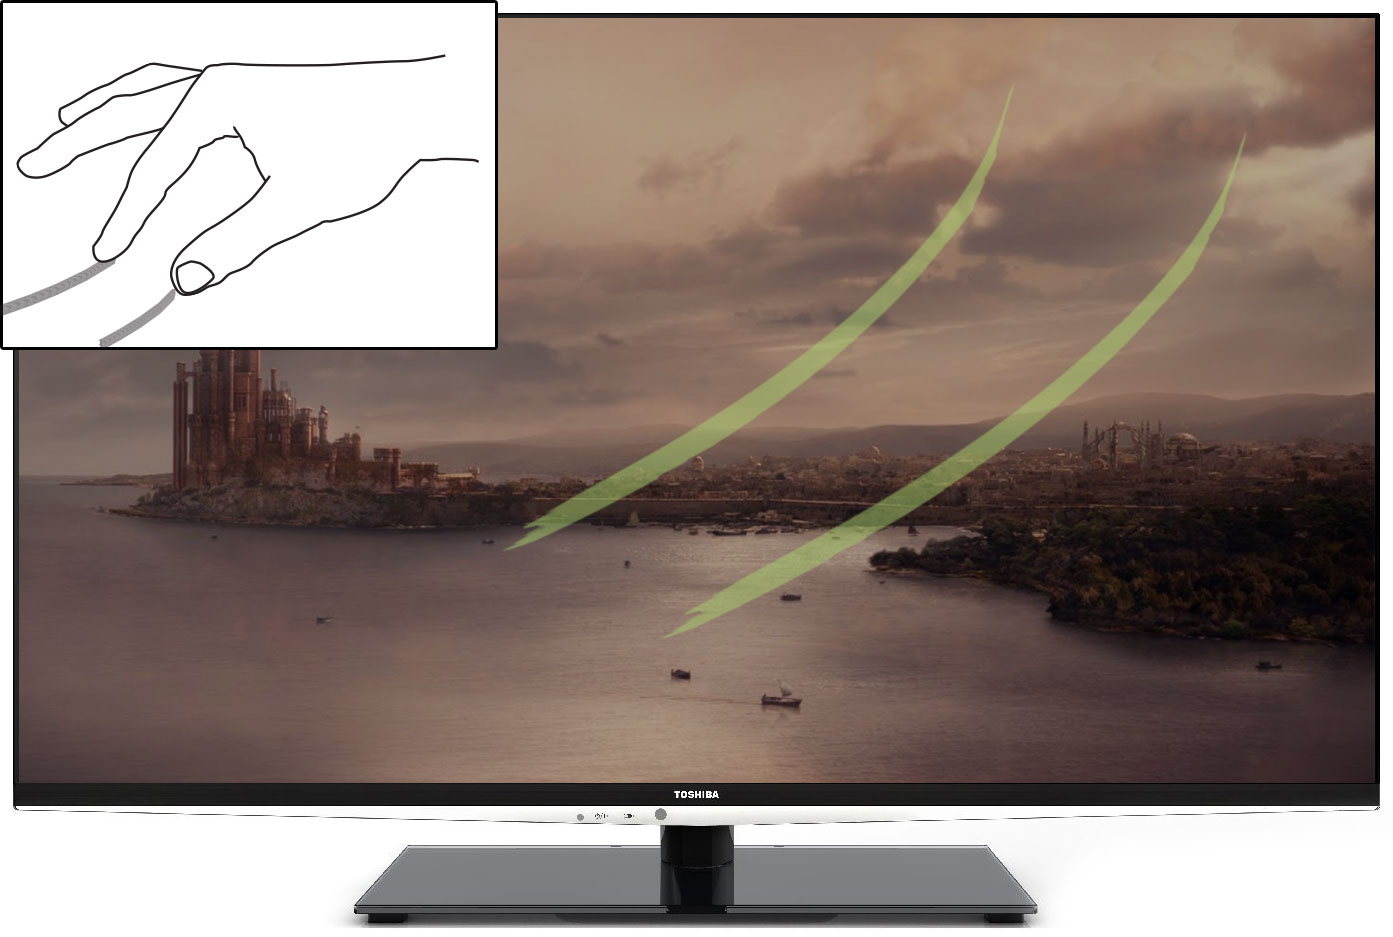
\includegraphics[width=\linewidth]{figures/touch/evaluation/gesture_overlay}
    \caption{The real-time overlay during touch. This ascending or descending two stroke gesture could for instance mean 'volume up' or 'down'.}
  \end{subfigure}%
  \hspace{0.02\textwidth}
  \begin{subfigure}[t]{.44\textwidth}
    \centering
    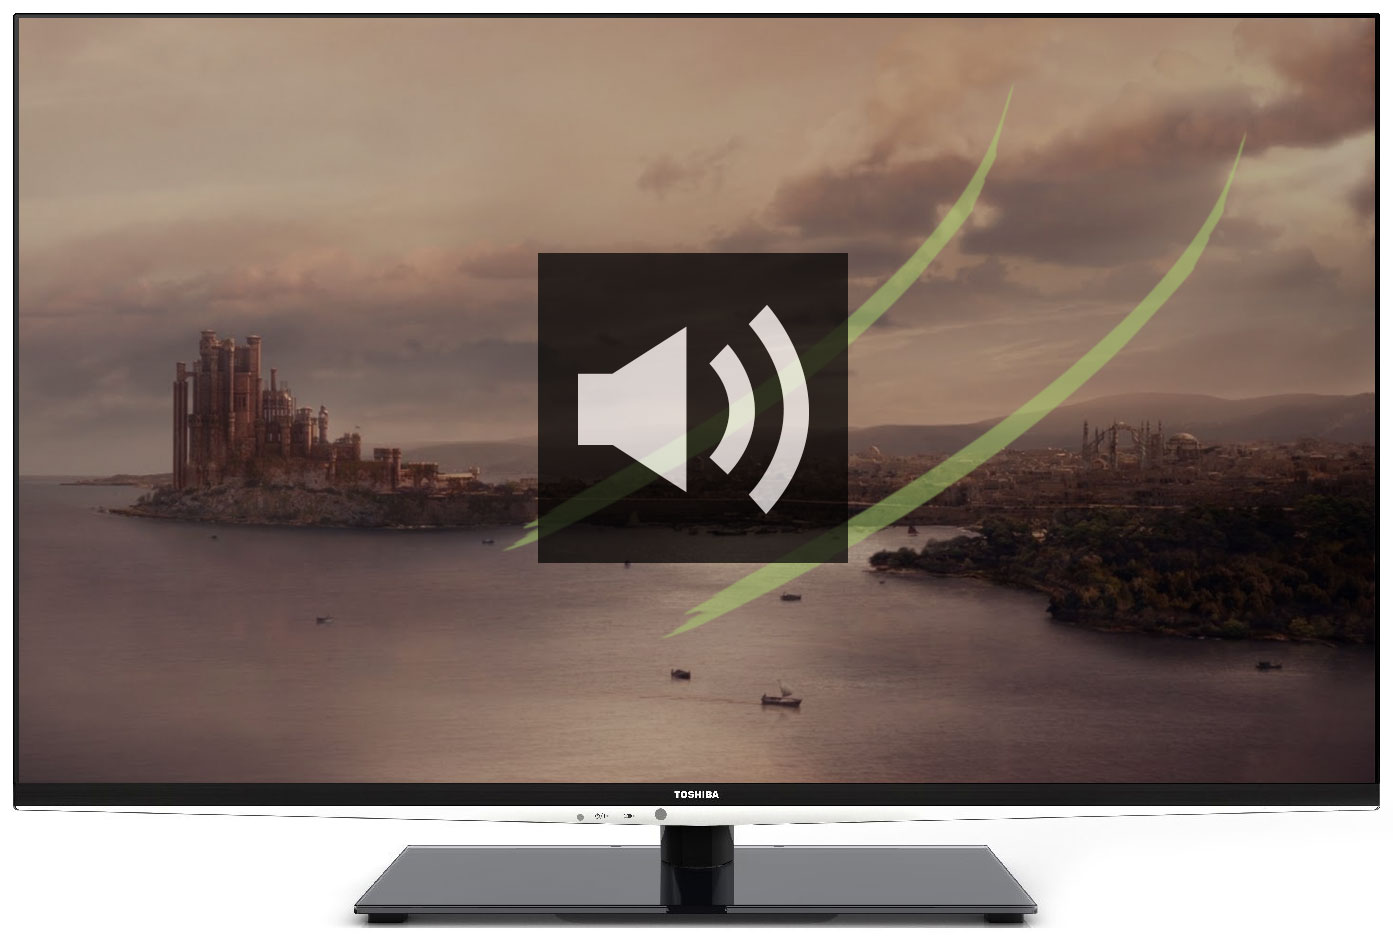
\includegraphics[width=\linewidth]{figures/touch/evaluation/gesture_overlay_2}
    \caption{The indication that a 'volume' action was performed.}
  \end{subfigure}
  \caption{Gesture input as an overlay for real-time feedback.}
  \label{fig:textiletouch:eval:overlay}
\end{figure}

\begin{figure}[h]
  \centering
  \begin{minipage}[b]{.8\textwidth}
    \centering
    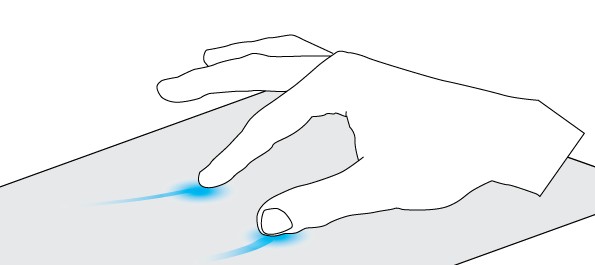
\includegraphics[width=.7\linewidth]{figures/touch/evaluation/backlid_textile}
  \caption[Illumination directly beneath touch points.]
  {Illumination directly beneath touch points.}
  \label{fig:textiletouch:eval:backlighting}
  \end{minipage}
\end{figure}

\begin{figure}
        \centering
        \begin{subfigure}[b]{0.44\textwidth}
                \centering
                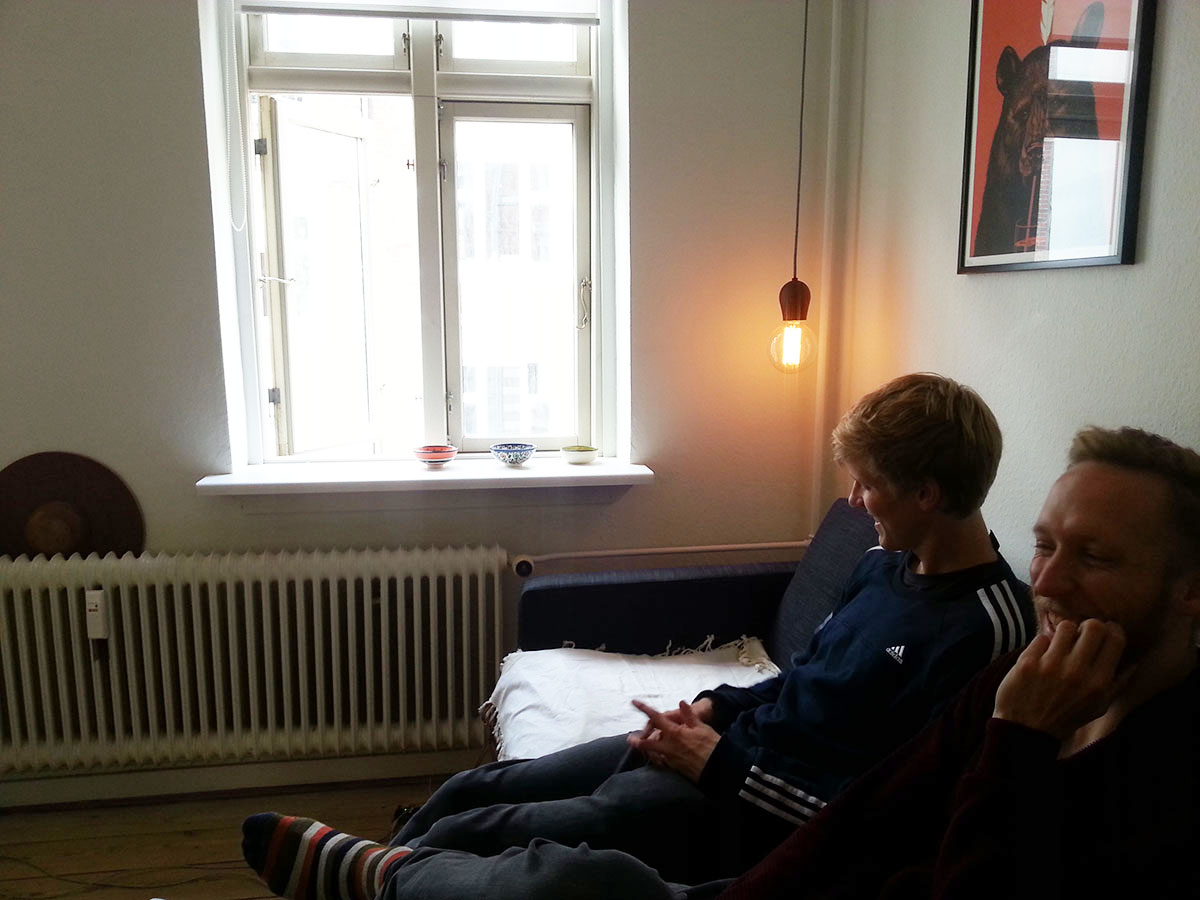
\includegraphics[width=\textwidth]{figures/touch/evaluation/sebastian/in_sofa}
                \caption{\dots}
                \label{fig:textiletouch:eval:sebastian:sofa}
        \end{subfigure}%
        \hspace{0.02\textwidth}
        \begin{subfigure}[b]{0.44\textwidth}
                \centering
                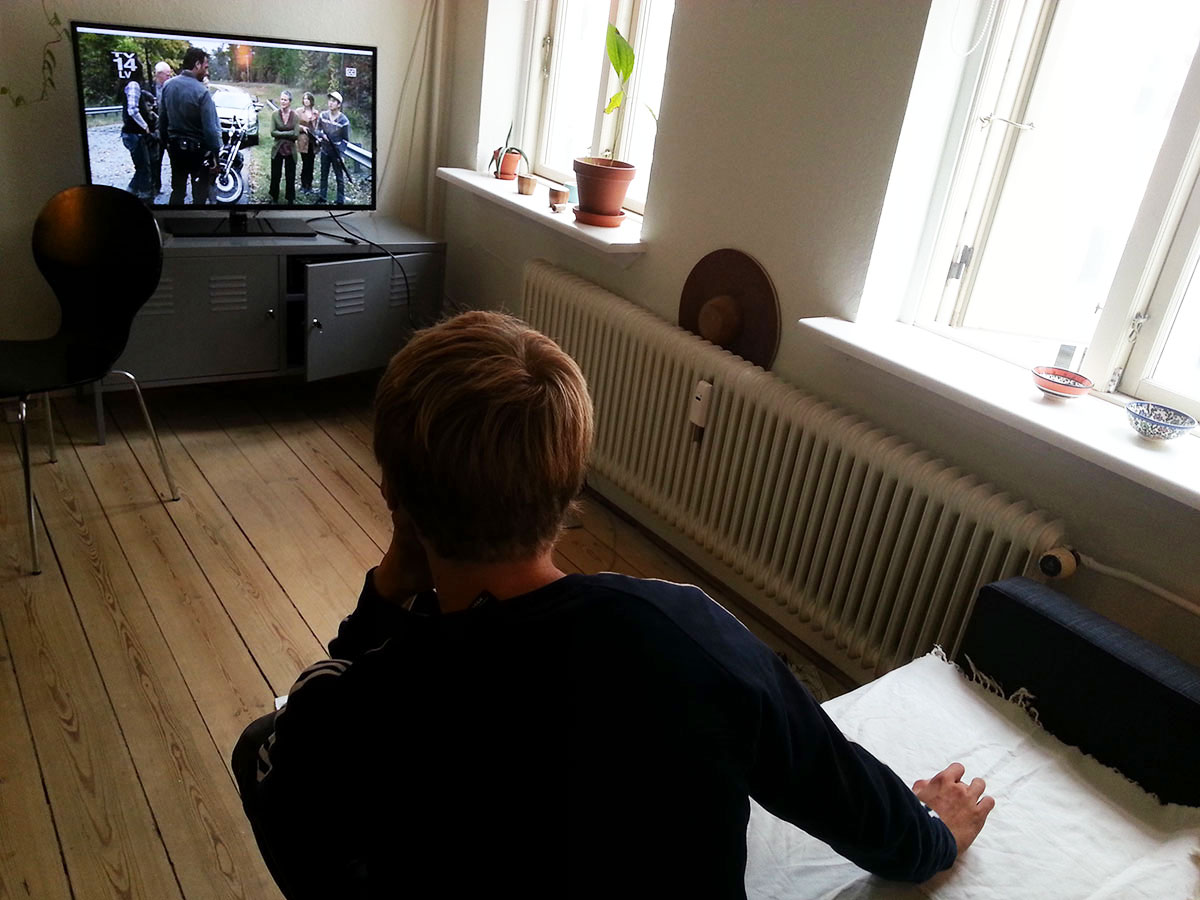
\includegraphics[width=\textwidth]{figures/touch/evaluation/sebastian/sofa_behind_seb}
                \caption{\dots}
                \label{fig:textiletouch:eval:sebastian:sofa_behind}
        \end{subfigure}

        \begin{subfigure}[b]{0.44\textwidth}
                \centering
                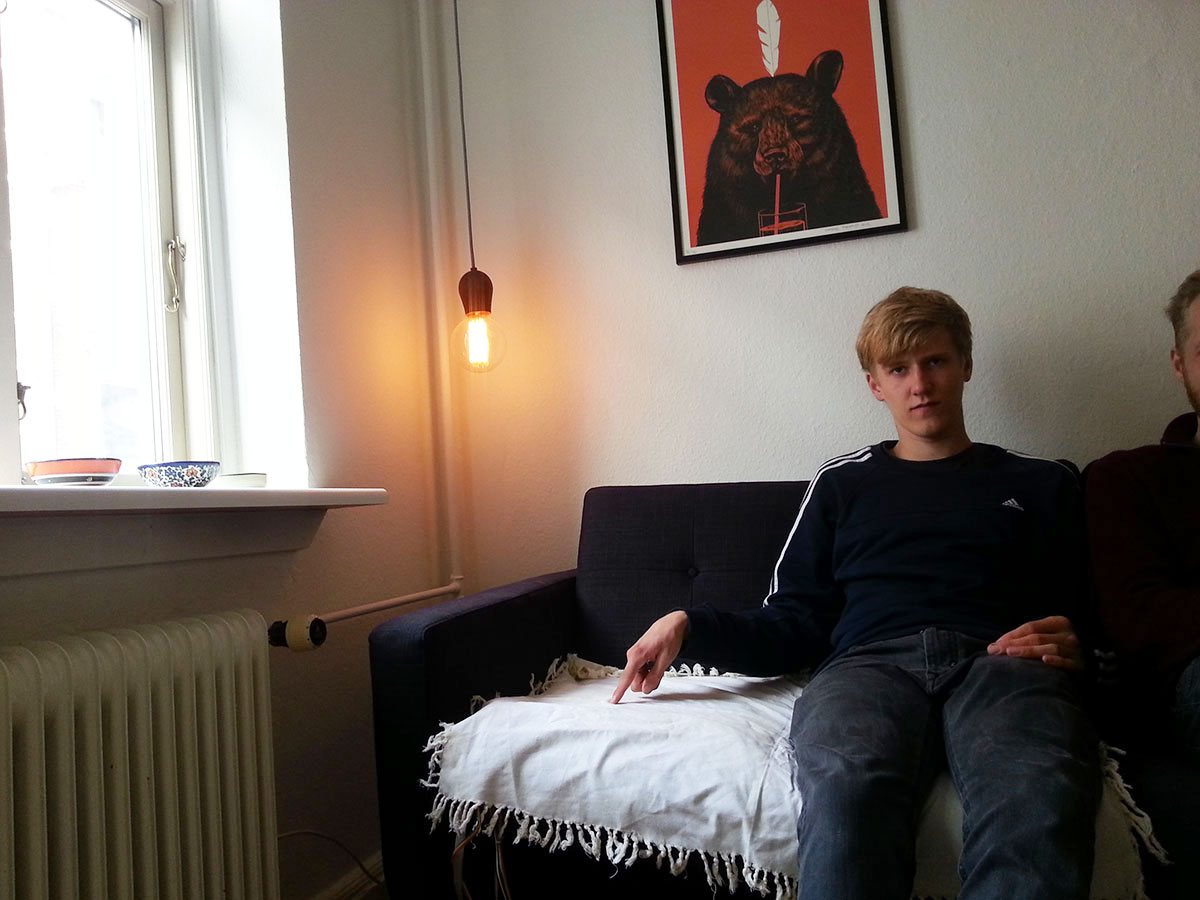
\includegraphics[width=\textwidth]{figures/touch/evaluation/sebastian/sofa_infront_seb}
                \caption{\dots}
                \label{fig:textiletouch:eval:sebastian:sofa_front}
        \end{subfigure}%
        \hspace{0.02\textwidth}
        \begin{subfigure}[b]{0.44\textwidth}
                \centering
                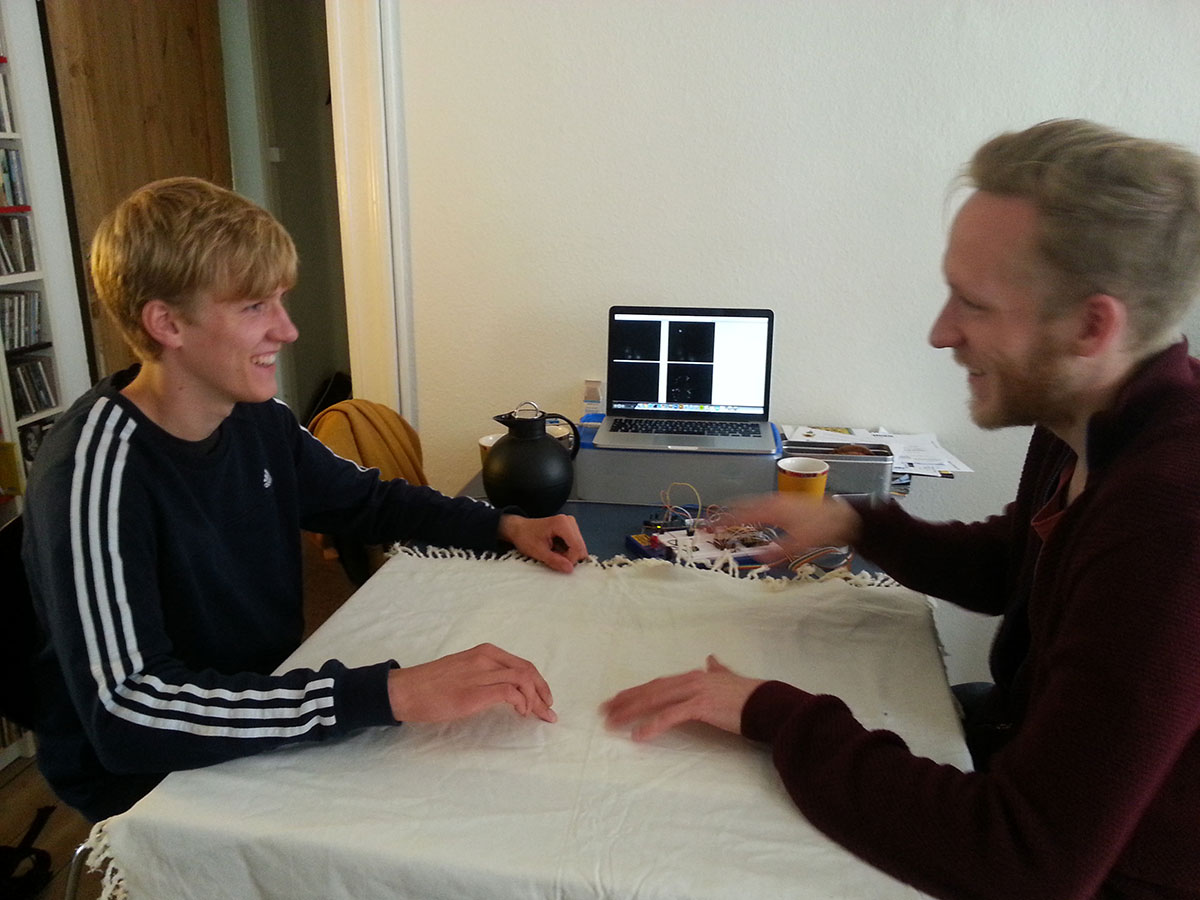
\includegraphics[width=\textwidth]{figures/touch/evaluation/sebastian/table}
                \caption{\dots}
                \label{fig:textiletouch:eval:sebastian:table}
        \end{subfigure}
        \caption{Teenager during evaluation \dots}
        \label{fig:textiletouch:eval:sebastian}
\end{figure}

\begin{figure}[h]
  \centering
  \begin{minipage}[b]{.8\textwidth}
    \centering
    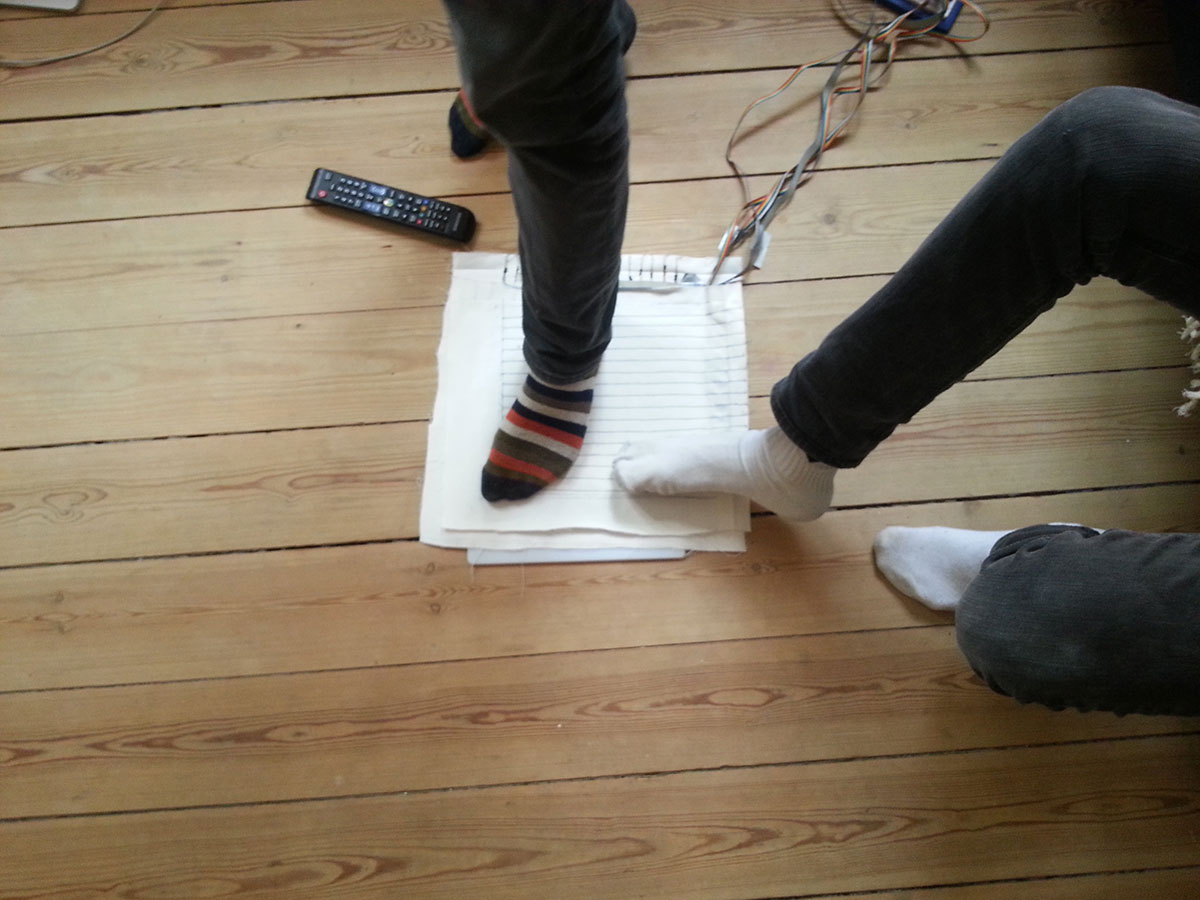
\includegraphics[width=.7\linewidth]{figures/touch/evaluation/sebastian/feet}
  \caption[Feet \dots]
  {Feet \dots}
  \label{fig:textiletouch:eval:sebastian:feet}
  \end{minipage}
\end{figure}

\begin{figure}
        \centering
        \begin{subfigure}[b]{0.44\textwidth}
                \centering
                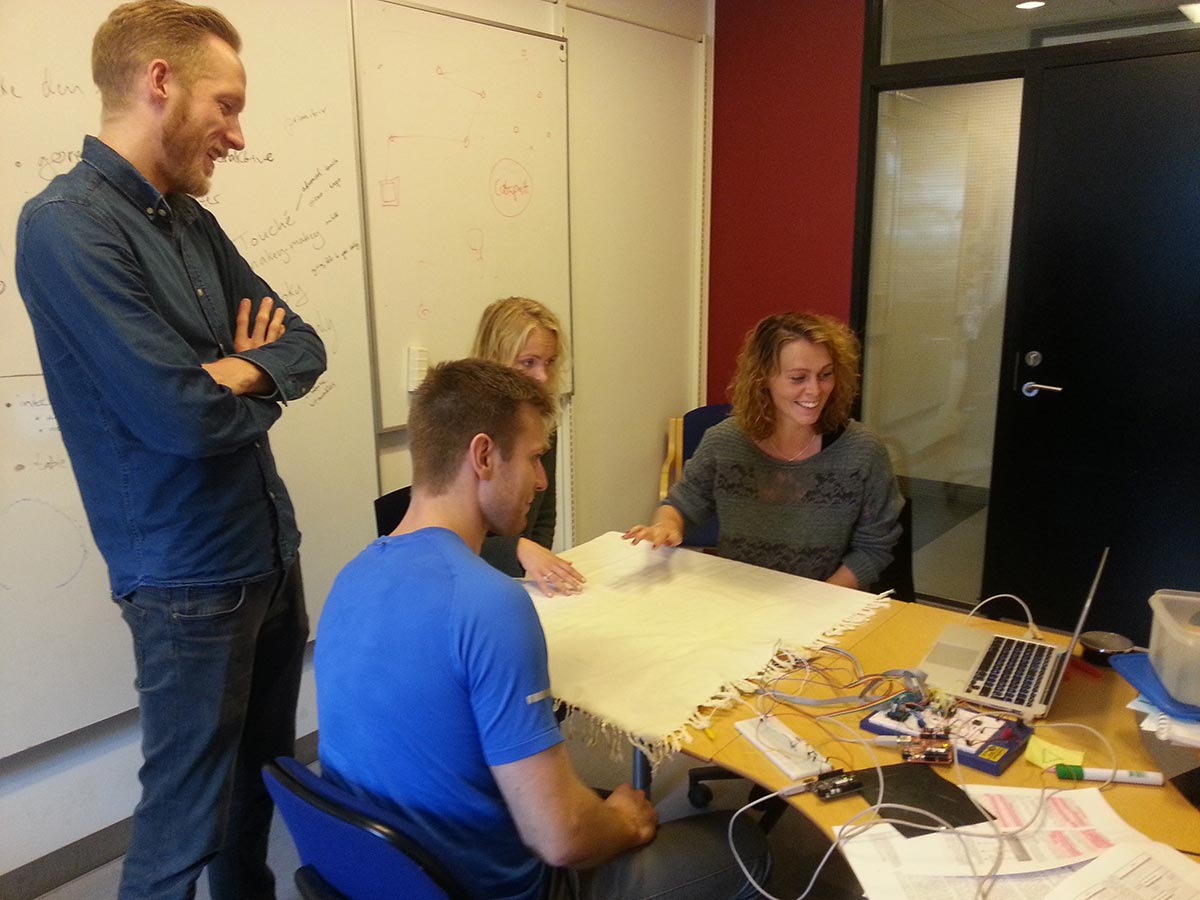
\includegraphics[width=\textwidth]{figures/touch/evaluation/kaia-gitte-troels/alle}
                \caption{\dots}
                \label{fig:textiletouch:eval:kaia-gitte-troels:alle}
        \end{subfigure}%
        \hspace{0.02\textwidth}
        \begin{subfigure}[b]{0.44\textwidth}
                \centering
                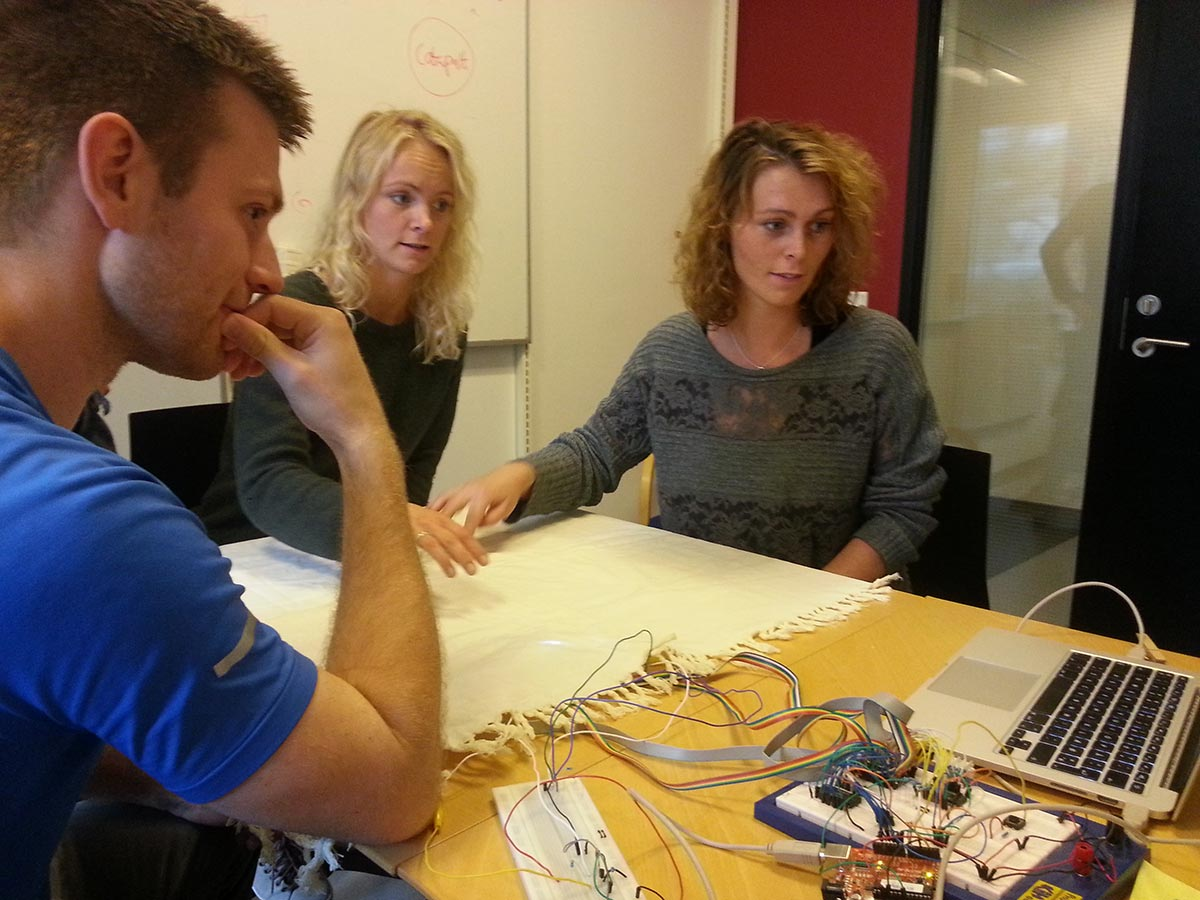
\includegraphics[width=\textwidth]{figures/touch/evaluation/kaia-gitte-troels/kaia-gitte2}
                \caption{\dots}
                \label{fig:textiletouch:eval:kaia-gitte-troels:kaia-gitte2}
        \end{subfigure}

        \begin{subfigure}[b]{0.9\textwidth}
                \centering
                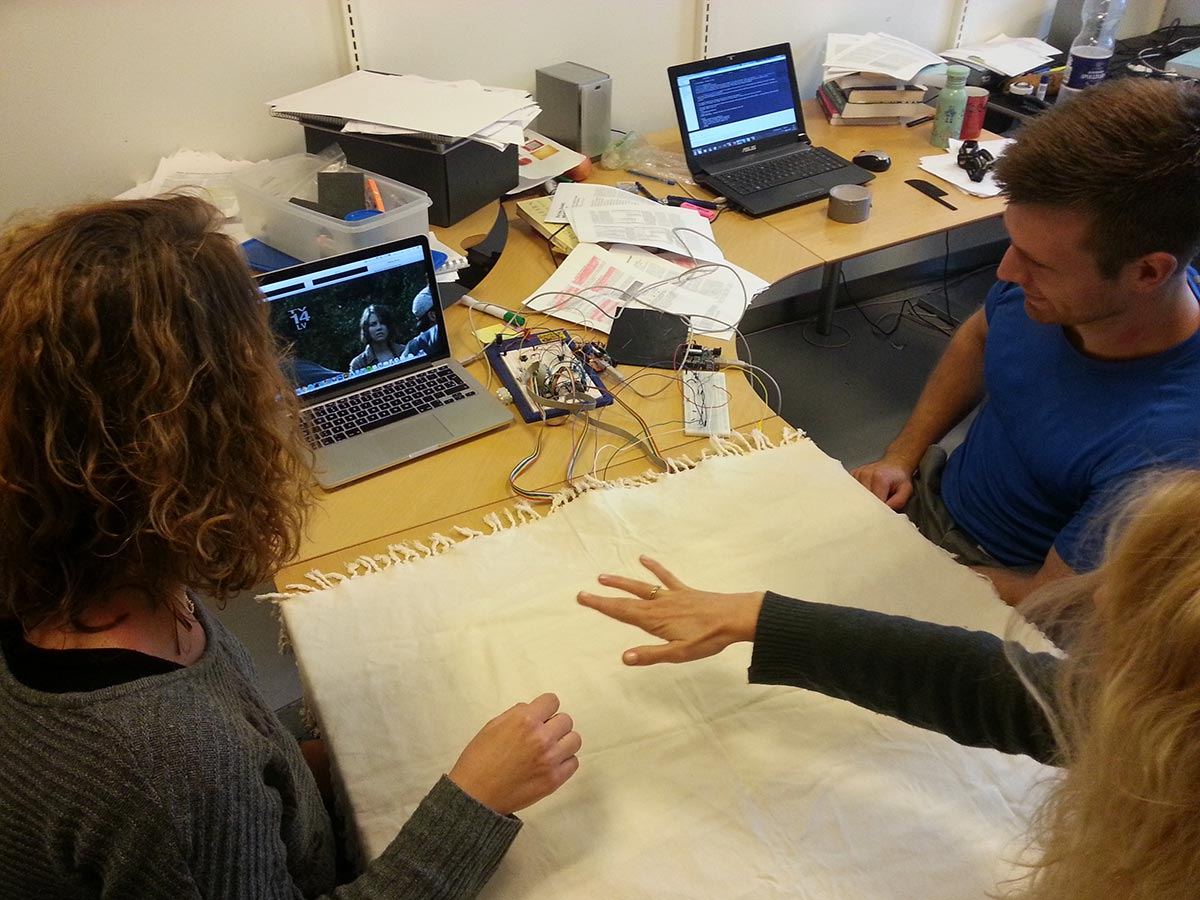
\includegraphics[width=\textwidth]{figures/touch/evaluation/kaia-gitte-troels/kaia-gitte}
                \caption{\dots}
                \label{fig:textiletouch:eval:kaia-gitte-troels:kaia-gitte}
        \end{subfigure}
        \caption{Teenager during evaluation \dots}
        \label{fig:textiletouch:eval:kaia-gitte-troels}
\end{figure}

\subsection{Potentials of alternative usages}

The ideas for alternative usages were in general very different from the idea of controlling existing devices.
The ideas were more characterised by sensor data being used in situations where meaning is open to interpretation as opposed to a one-to-one mapping between input gesture and function.
For example, several ideas concerning safety and security were discussed.

% toddlers
Parents of toddlers often have floor mats for their child to lay and play on, see figure~\ref{fig:textiletouch:eval:softtiles}.
Instead of having parents checking up on their child every two minutes these mats could have touch fields embedded.
The sensor data can then be abstracted to inform parents about the activity of their child by recording pressure and movement, giving the concerned parent room to do less frequent check ups.
This is actually a very simple setup that does not require a high resolution of the sensor grid and the output required could be condensed to simple states such as, whether the toddler is on the mat and the level of movement activity.

% elders
Elderly people with a weak physic or people with Parkinson's disease have a tendency to fall over easily.
One of the approaches in reducing the consequences of a fall is to give the elders assistive devices such as wearable fall detectors which can automatically release an alarm in the event of a fall.
An alternative approach, which does not require body equipment, could be to prepare the home with sensitive impact sensitive floors or carpets.
Some may base their sense of security in a physical wearable device while others find it inconvenient, a source of irritation, or maybe even an exceedance of personal privacy. 
With safety measurements invisibly integrated into the home the sense of security may be directed towards to the scope of the home as a whole.

% handicap
Some disabled people with hindered mobility 
\blank
% Home security
During the evaluations we also discussed a scenario of home security regarding the front door of ones home.
In this scenario we imagined a blank door with no handle and no lock and thereby no need for a key.
Instead the door had an embedded grid of pressure sensors.
We came up with and enacted two different interaction styles for opening the door.
One was a variant of the pattern lock found in many Android smart phones where a set of points must be touched in the correct sequence in order for the door to unlock, see figure \todo{billede af Kaia og Gitte ved doeren 1}.
The other was based on the fact that people have unique signatures which could be used for authentication.
A person would then have to makes strokes (the signature) on the door facade to be authenticated and have the door unlock and open, see figure \todo{billede af Kaia og Gitte ved doeren 2}.

This is a good example of an ad hoc interface \emph{through invisible interfaces embedded into the physical environment}.
Knowledge of the system is a prerequisite to enter in that you are faced with a blank facade with no direct indication of how to enter.
It also confronts the raised issue of invisible interfaces and affordances by using it as an advantage in a security setting where the absence of a lock and door handle would inhibit a trespasser.
\blank
% Sleep cycle
Moving away from the topic of safety and security and to the topic of self-tracking, a movement that has gained a lot popularity in recent years with the advent of consumer gadgets, such as Fitbit\footnote{http://www.fitbit.com/}, Nike+\footnote{http://nikeplus.nike.com/plus/} and loads more. 
These gadgets let you sense just about anything concerning your body, quantifying yourself in numbers.
An example of this is sleep monitoring and optimisation, which in its simplest form only requires a smart phone next to your body in bed, but can take on more advanced forms as well with a variety of body sensors.
With a smart phone the approach is to use the built-in accelerometer to detect movement during sleep to graph the total sleep and derive whether the person is in deep sleep or light sleep.
These data can also be used to trigger the wake-up alarm at moments of light sleep within a specified time frame close to the set alarm time.

A product with the capabilities of our textile touch prototype which can infer the same kind information by the means of a pressure measurements over time, would be an interesting alternative.
Being integrated as part of a madras or a bed sheet it would be unnoticeable for a sleeping person and would not require a smart phone next to the pillow which some may be precautious about.

This application does not really fall under the category of AHIs, but it is mentioned here for the potential of a discrete and unobtrusive product as a continuation of the self-tracking movement.


\begin{figure}[h]
  \centering
  \begin{minipage}[b]{.8\textwidth}
    \centering
    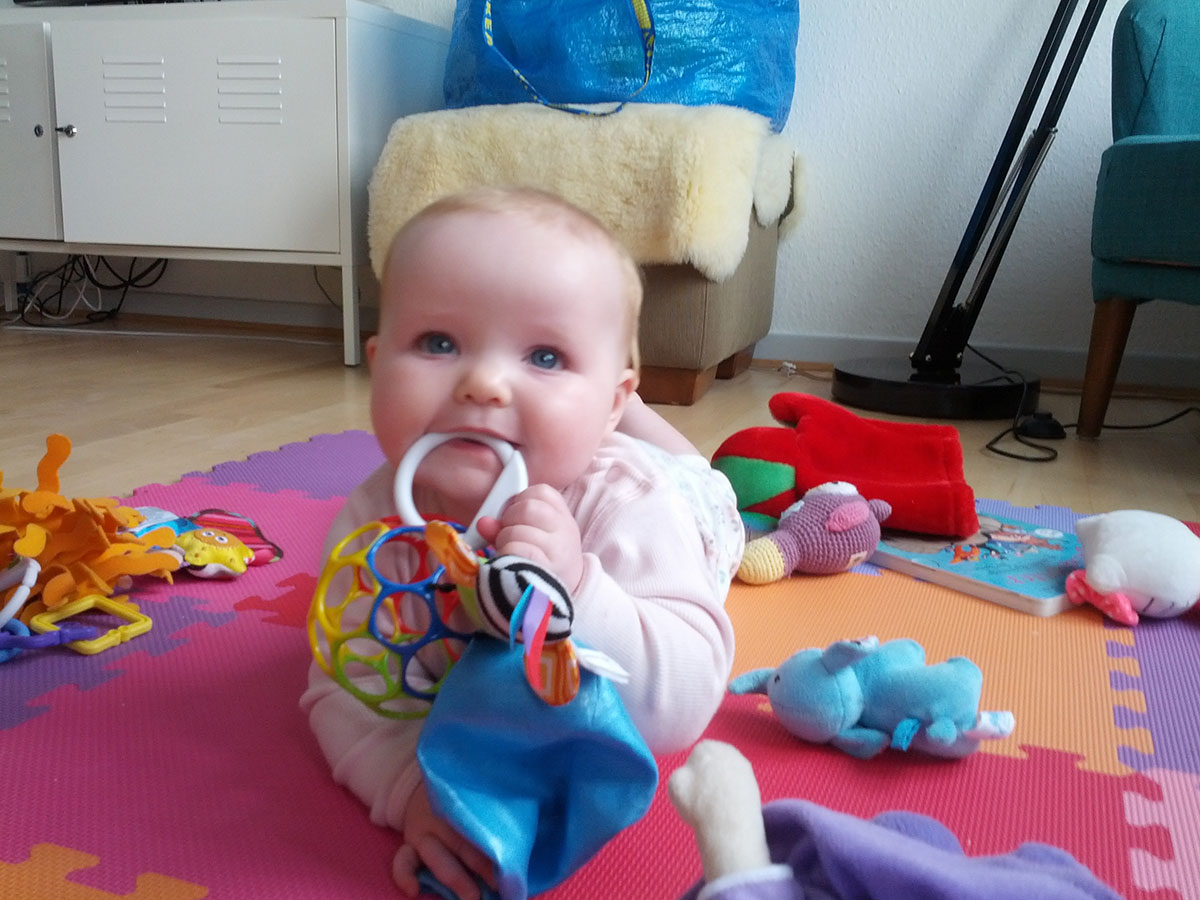
\includegraphics[width=.7\linewidth]{figures/touch/evaluation/softtiles}
  \caption[Toddler on a foam floor mat with puzzle-like tiles for extensibility.]
  {Toddler on a foam floor mat.}
  \label{fig:textiletouch:eval:softtiles}
  \end{minipage}
\end{figure}

\begin{verbatim}
**** Paw + Morten ****
* tegning paa overflader: "hvis danmark nu er her ... og holland her, saa ..." 
	- for at forklare ting.
* boernevaerelse - legemaatte, hvor foraeldre kan se aktivitetsniveau for 
	deres unger og dermed ikke behoever at tjekke op paa dem hele tiden.
* handikaphjem
	* vildt mange ting der skal styres
    * mobilitet er begraenset
* aeldrehjem
    * crash taeppe - folk med parkison der ofte vaelter eller lign.
        * eller alle flader
    * "hvis man ikke har noget paa kan det ikke tages" - nuvaerende situation 
		hvor aeldre faar "halsbaand" (falde-detektor) paa, som de tager af i tide og utide.
* Sikkerhed. Den usynlig noegle - man skal vide hvor man input delen er for 
	at kunne lave en "adgangsgestik".
    * Eller det, at mennesker har en unik "haandskrift" der kan anvendes 
		paa touch overfladen.
    * doermaatte
\end{verbatim}

\subsection{Future work}
\label{ch:textiletouch:futurework}

There are several points about the prototype that are candidates for future work.

% Multitouch
On the technical side there is room for improvement.
As the technology allows for multi-touch input it would be a great improvement for the user experience.
Multi-touch provides a much richer interaction style \todo{reference?} compared to single-touch and has become a standard in modern smart phone displays and laptop touchpads, most notably for scrolling, zooming and rotation.
The gesture recognition framework used for the prototype, \$P, will work just fine with multi-touch and will not require further adjustment as the method of input is totally decoupled from the recognition framework. \todo{though gestures or symbols are not the same as real-time gestures on a mouse-pad such as zooming}
Instead it is our peak detection algorithms that need to be reimplemented and take multiple peaks in to account.
Figure~\todo{ref} shows a frame of input where several peaks made by finger inputs are detected. \todo{provide reason for not implementing multi-touch in the firstplace?}

As can be seen in the figure every peak is surrounded by some noise created by finger pressure propagating away from the peak spot.
It should be noted that we do not consider values in the immediate proximity of a peak to be noise as we use these values to make interpolation and thereby scale the resolution by a factor a 10.
We have already taken steps to reduce this by implementing a simple averaging filter in the software 
where a sample is an average of \emph{x} previous samples.
There are also steps to be taken on the hardware side where a noise filter could reduce the signal-to-noise ratio before entering the software part.

\todo{ting der er belyst fra evaluering \dots}

\begin{verbatim}
dette er ikke faerdig prototype - snakke om forskellige retninger
Real-world implementation - e.g. a whole sofa, wall paper?
\end{verbatim}

